\documentclass[defaultstyle,10pt,master,Helvetica]{01.thesis}
%Use 01.thesis_pt instead for PT version 
%Dummy text if written by default in English. Just changed to whatever you need.
% Helvetica is a similar font to Arial, with small differences.

%% Packages
\typeout{}
\typeout{--------------------------------------------------------------}
\typeout{ +---+ Thesis Template                            }
\typeout{ +---+      Version 1.7.8, April 2016                         }
\typeout{ +---+  for Instituto Superior Tecnico (IST),                 }
\typeout{ +---+  Universidade Técnica de Lisboa                         }
\typeout{ * Using Thesis Style from Pedro Tomás                                }
\typeout{ * Created to write Dissertations                             }
\typeout{ * Conforms with IST Master Degree format and with most important packages setup        }
\typeout{ * Should conform with IST PhD Degree format (not verified)   }
\typeout{                                                              }
\typeout{ AUTHOR: Miguel Amador and João Marques                                          }
\typeout{                                                              }
\typeout{Important: Use all files in the archive, since this is based in all them. Modify dummy files at wish.                                                              }
\typeout{--------------------------------------------------------------}
\typeout{}

% MY OWN PACKAGES
\usepackage{cuted}
\usepackage{bm}
\usepackage{bbm}
\usepackage{setspace}
\pagenumbering{arabic}
\usepackage{scrextend}
\usepackage{ragged2e}
\usepackage{xcolor}
\usepackage{dirtytalk}

% Defines an additional alphabet... not required in most cases
% ------------------------------------------------------------
% \DeclareMathAlphabet{\mathpzc}{OT1}{pzc}{m}{it}

% PACKAGE babel:
% ---------------
% The 'babel' package may correct some hyphenisation issues of latex. 
% However in most situations it is not required.
\usepackage[portuguese,english]{babel}


% PACKAGE fontenc:
% -----------------
% chooses T1-fonts and allows correct automatic hyphenation.
%\usepackage[T1]{fontenc}
%\usepackage[latin1]{inputenc}
\usepackage[utf8]{inputenc}
\usepackage[T1]{fontenc}
%\usepackage{lmodern} %will change font type

% Package ulem.
\usepackage{ulem} % Allows the use of other text emphatizer commands
\normalem %defines \emph{} to italic, instead of underline. 
\raggedbottom %declaration makes all pages the height of the text on that page. No extra vertical space is added. The \flushbottom declaration makes all text pages the same height, adding extra vertical space when necessary to fill out the page.

% PACKAGE date time:
% -----------------
% Lets you alter the format of the date that \today returns.
\usepackage{datetime}
\newdateformat{todaythesis}{%
\monthname[\THEMONTH]  \THEYEAR}

% PACKAGE latexsym:
% -----------------
% Defines additional latex symbols. May be required for thesis with many math symbols.
\usepackage{latexsym}

% PACKAGE amsmath, amsthm, amssymb, amsfonts:
% -------------------------------------------
% This package is typically required. Among many other things it adds the possibility
% to put symbols in bold by using \boldsymbol (not \mathbf); defines additional 
% fonts and symbols; adds the \eqref command for citing equations. I prefer the style
% "(x.xx)" for referering to an equation than to use "equation x.xx".
\usepackage{amsmath, amsthm, amssymb, amsfonts, amsbsy}

% PACKAGE multirow, colortbl, longtable:
% ---------------------------------------
% These packages are most usefull for advanced tables. The first allows to join rows 
% throuhg the command \multirow which works similarly with the command \multicolumn
% The second package allows to color the table (both foreground and background)
% The third package is only required when tables extend beyond the length of one page;
% with compatibilities with the tabular environment. The last allow the definitions of landscape pages, allowing the use of a different orientation for wider graphics or tables. See package documentation to see the implementation.
\usepackage{multirow}
\usepackage{colortbl}
\usepackage{supertabular}
\usepackage{pdflscape}
% \usepackage{longtable}

% PACKAGE graphics, epsfig, subfigure, caption:
% ---------------------------------------------
% Packages for figures... well you will certainly need these packages, with the exception
% of the 'caption' package. This only allows to define extra caption options.
% Notice that subfigure allows to place figures within figures with its own caption. It
% should be avoided to create an eps file with subfigures. That will mean that you won't be 
% able to reference those subfigures. Instead create an EPS file (the only graphics format supported
% by latex) for each of the subfigures and then use the command \subfigure (see below).
\usepackage{graphics}
\usepackage{graphicx}
\usepackage{epsfig}
\usepackage[hang,small,bf]{subfigure}
%\usepackage[footnotesize,bf,center]{caption}
\usepackage{dcolumn}
\usepackage{bm}
\usepackage{booktabs}
\usepackage{rotating}
\usepackage{multirow}

\usepackage[font=small,labelfont=bf,textfont=normalfont]{caption}

% PACKAGE algorithmic, algorithm
% ------------------------------
% These packages are required if you need to describe an algorithm.
 \usepackage{algorithmic}
 \usepackage[chapter]{algorithm}

% PACKAGE natbib/cite/biblatex
% -------------------
% The three packages are not compatible, and you should use one of the two. Notice however that the
% IEEE BiBTeX stylesheet is imcompatible with the natbib package. If using the IEEE format, use the 
% cite package instead
%% Natbib
\usepackage[square,numbers,sort&compress]{natbib}
%% Cite
%\usepackage{cite}
%% Biblatex (Not working)
%\usepackage{csquotes}
%\usepackage[backend=biber,style=authoryear]{biblatex}


% PACKAGE acronyum
% -----------------
% This package is most useful for acronyms. The package guarantees that all acronyms definitions are 
% given at the first usage. IMPORTANT: do not use acronyms in titles/captions; otherwise the definition 
% will appear on the table of contents.
\usepackage[printonlyused]{acronym}
\usepackage[titletoc,title,header]{appendix}
\usepackage[noauto]{chappg}
%The following line assures that each chapter deals with acronyms idependently.
%You may also do it manually by calling acresetall anywhere in the documento to reset the acronyms behaviour. 
\preto\chapter\acresetall

% PACKAGE extra_functions VER COMO DEVE SER
% -----------------
% My Personal package: defines the following commands:
% \fancychapter{chaptername) -> Prints a fancier chapter (you can also use the fancychapter package for this)
% \hline{width} -> use for a replacement of the \hline command
% \Mark1, \Mark2, \Mark3, ...
\usepackage{00.extra_functions}


% PACKAGE hyperref
% -----------------
% Set links for references and citations in document
% Some MiKTeX distributions have faulty PDF creators in which case this package will not work correctly
% Long live Linux :D
\usepackage[plainpages=false]{hyperref}
\hypersetup{
             colorlinks=false,
             citecolor=red,
             breaklinks=true,
             bookmarksnumbered=true,
             bookmarksopen=true,
             pdftitle={Thesis Title},
             pdfauthor={Author Name},
             pdfsubject={Master Thesis in Biomedical Engineering},
             pdfcreator={Document Creator Name},
             pdfkeywords={Template, Latex, Thesis}}
\usepackage{float}
\usepackage{url}
%\usepackage[final]{00.listofsymbols}
\usepackage{00.symlist}

% Set paragraph counter to alphanumeric mode
\renewcommand{\theparagraph}{\Alph{paragraph}~--}

\newcommand{\figref}[1]{Figure \ref{#1}}
\newcommand{\equationref}[1]{Equation (\ref{#1})}
\newcommand{\tableref}[1]{Table (\ref{#1})}

\newcommand{\textreg}{$\textsuperscript{\textregistered}$}


%% Page formatting
\hoffset 0in
\voffset 0in

%Alternative set of page geometry
%\oddsidemargin 0.71cm
%\evensidemargin 0.04cm
%\marginparsep 0in
%\topmargin -0.25cm
%\textwidth 15cm
%\textheight 23.5cm

\usepackage[top=2.5cm, bottom=2.5cm, inner=2.9cm, outer=2.5cm]{geometry}

\usepackage{fancyhdr}
\pagestyle{fancy}
\renewcommand{\chaptermark}[1]{\markboth{\thechapter.\ #1}{}}
\renewcommand{\sectionmark}[1]{\markright{\thesection\ #1}}
\fancyhf{} 
%\fancyhead[LE]{\bfseries\nouppercase{\leftmark}}
%\fancyhead[RO]{\bfseries\nouppercase{\rightmark}}
\fancyfoot[LE,RO]{\bfseries\small\thepage}
\renewcommand{\headrulewidth}{0.0pt}
\renewcommand{\footrulewidth}{0.0pt}
\addtolength{\headheight}{2pt} % make space for the rule
\fancypagestyle{plain}{% Used in Chapter titles
   \fancyhead{} % get rid of headers
   \renewcommand{\headrulewidth}{0pt} % and the line
   \renewcommand{\footrulewidth}{0pt}
   \fancyfoot[LE,RO]{\bfseries\small\thepage}
}

\fancypagestyle{begin}{%
   \fancyhead{}
   \renewcommand{\headrulewidth}{0pt}
   \renewcommand{\footrulewidth}{0pt}
   \fancyfoot[LE,RO]{\bfseries\small\thepage}
}
\fancypagestyle{document}{%
	\fancyhf{} 
	\fancyhead[LE]{\bfseries\nouppercase{\leftmark}}
	\fancyhead[RO]{\bfseries\nouppercase{\rightmark}}
	\fancyfoot[LE,RO]{\bfseries\small\thepage}
	%\renewcommand{\headrulewidth}{0pt}
	%\renewcommand{\footrulewidth}{0pt}
	\addtolength{\headheight}{2pt} % make space for the rule
}
\fancypagestyle{documentsimple}{%
	\fancyhf{}
	\fancyfoot[LE,RO]{\bfseries\small\thepage}
	%\renewcommand{\headrulewidth}{0pt}
	%\renewcommand{\footrulewidth}{0pt}
	\addtolength{\headheight}{2pt} % make space for the rule
}
\setcounter{secnumdepth} {5}
\setcounter{tocdepth} {5}
\renewcommand{\thesubsubsection}{\thesubsection.\Alph{subsubsection}}

\renewcommand{\subfigtopskip}{0.3 cm}
\renewcommand{\subfigbottomskip}{0.2 cm}
\renewcommand{\subfigcapskip}{0.3 cm}
\renewcommand{\subfigcapmargin}{0.2 cm}

\graphicspath{{Figures/}}



%-----------------------------------------------------------
%-----------------------------------------------------------
\begin{document}
%% Use Main document Language
\selectlanguage{english}
%% ------
\pagestyle{begin}
\setcounter{page}{1} \pagenumbering{Alph}

% Add PDF bookmark 
\pdfbookmark[0]{Title}{Title}

\thispagestyle{empty}

\begin{flushleft} ~\\ \vspace{-12mm} \hspace{-12mm}

\includegraphics[width=50mm]{Cover/istnewlogo}
\vspace{10mm}
%~\\ \vspace{50mm} % gráficos
\\ \begin{center} 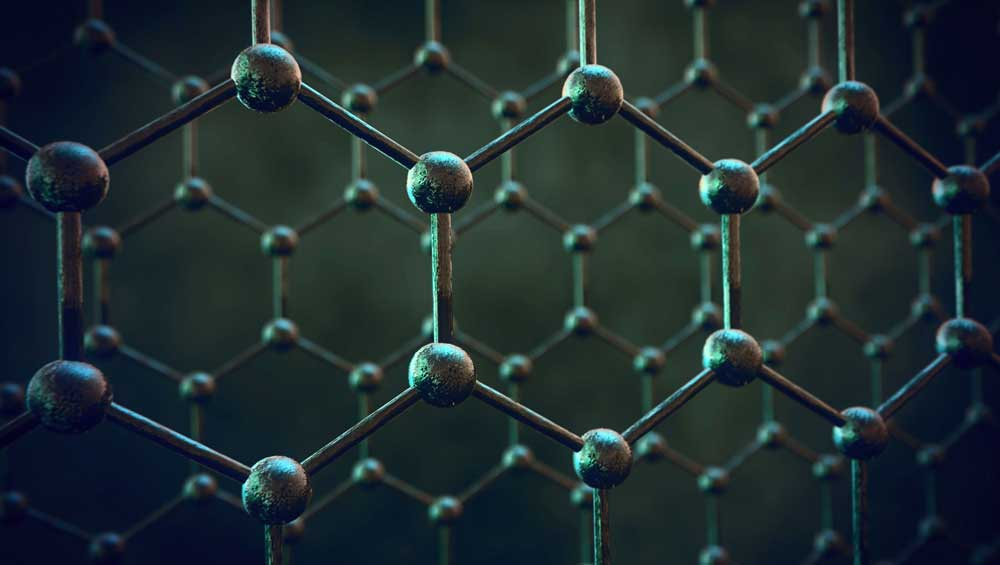
\includegraphics[height=50mm]{Cover/coverimage}  \end{center} % gráficos
 \vspace{5mm}
\centering
\LARGE \textbf{Development of a QMC code to tackle interacting electronic systems in 2D with application to TMD nanoribbons}
\\
\vspace{15mm}
\Large \textbf{Francisco Monteiro de Oliveira Brito} \\
\vspace{12mm}
\large Thesis to obtain the Master of Science Degree in
\\ \vspace{2mm}
\LARGE \textbf{Physics Engineering}
\\ \vspace{10mm}
\large Supervisor(s): Prof. João Manuel Viana Parente Lopes  \\
\large Prof. Eduardo Filipe Vieira de Castro
\\ \vspace{15mm}
\Large \textbf{Examination Committee}
\\ \vspace{5mm}
\large Chairperson:	Prof. Lorem \\
\large Supervisor: Prof. João Manuel Viana Parente Lopes\\
\large Co-Supervisor: Prof. Eduardo Filipe Vieira de Castro \\
\large Members of the Committee: Dr. Lorem Ipsum \\
Prof. Lorem Ipsum
 
\vspace{15mm}

\Large \textbf{\todaythesis\today} \\
\let\thepage\relax
\end{flushleft}
\pagebreak


\clearpage
% Since I am using double sided pages, the second page should be white.
% Remember that when delivering the dissertation, IST requires for the cover to appear twice.

\thispagestyle{empty}
\cleardoublepage

\setcounter{page}{1} \pagenumbering{roman}

\baselineskip 18pt % line spacing: -12pt for single spacing
                   %               -18pt for 1 1/2 spacing
                   %               -24pt for double spacingnts}
 
\thispagestyle{empty}
\hbox{} \vfill
\begin{flushright}
\small \textit{\textbf{The behavior of large and complex aggregates of elementary particles, it turns out, is not to be understood in terms of a simple extrapolation of the properties of a few particles.}}
\\ \vspace{2mm}  
\scriptsize P. W. Anderson
\end{flushright}

\clearpage
\thispagestyle{empty}
\cleardoublepage

\pdfbookmark{Acknowledgments}{Acknowledgments}
\begin{acknowledgments} 

I would like to thank the Academy, bla bla bla..

\end{acknowledgments}
\clearpage
\thispagestyle{empty}
\cleardoublepage
\selectlanguage{english}
\begin{abstract}

The Objective of this Work ... (English)

\end{abstract}
\begin{keywords}
Keywords (English)
\end{keywords}
\clearpage
\thispagestyle{empty}
\cleardoublepage
\selectlanguage{portuguese}
\begin{resumo}

O objectivo deste trabalho ... (Português)

\end{resumo}
\begin{palavraschave}
Palavras-Chave (Português)
\end{palavraschave}
\clearpage
\thispagestyle{empty}
\cleardoublepage
%% Use Main document Language
\selectlanguage{english}
%% ------
% This is required for the fancy chapters
\dominitoc
\dominilof
\dominilot

%%%%%%%%%%%%%%%%%%%%%%%%%%%%%%%%%%%%%%%%%%%%%%%%%%%%%%%%%%%%%%%%%%%%%%
% List of contents
%\renewcommand{\baselinestretch}{1}
\pdfbookmark[0]{Index}{index}
\pdfbookmark[1]{Contents}{toc}
\tableofcontents
% \contentsline{chapter}{References}{\pageref{bib}}
\clearpage
\thispagestyle{empty}
\cleardoublepage
%\renewcommand{\baselinestretch}{1.5}
%%%%%%%%%%%%%%%%%%%%%%%%%%%%%%%%%%%%%%%%%%%%%%%%%%%%%%%%%%%%%%%%%%%%%%
% List of figures
\pdfbookmark[1]{List of Figures}{lof}
\listoffigures
\clearpage
\thispagestyle{empty}
\cleardoublepage

%%%%%%%%%%%%%%%%%%%%%%%%%%%%%%%%%%%%%%%%%%%%%%%%%%%%%%%%%%%%%%%%%%%%%%
% List of tables
\pdfbookmark[1]{List of Tables}{lot}
\listoftables
\clearpage
\thispagestyle{empty}
\cleardoublepage

% %%%%%%%%%%%%%%%%%%%%%%%%%%%%%%%%%%%%%%%%%%%%%%%%%%%%%%%%%%%%%%%%%%%%%%
% % List of algorithms
% Requires packages algorithmic, algorithm
% \pdfbookmark[1]{List of Algorithms}{loa}
% \listofalgorithms
% \cleardoublepage
\acresetall
%% Remain list of table titles are set manualy
% %%%%%%%%%%%%%%%%%%%%%%%%%%%%%%%%%%%%%%%%%%%%%%%%%%%%%%%%%%%%%%%%%%%%%%
 % List of acronyms
\pdfbookmark[1]{List of Acronyms}{loac}

\chapter*{Abbreviations}


% See more at http://staff.science.uva.nl/~polko/HOWTO/LATEX/acronym.html

\begin{acronym}
\acro{acro}{Dummy Acronym}
\end{acronym}

\clearpage
\thispagestyle{empty}
\cleardoublepage




%%%%%%%%%%%%%%%%%%%%%%%%%%%%%%%%%%%%%%%%%%%%%%%%%%%%%%%%%%%%%%%%%%%%%%
% List of symbols
\pdfbookmark[1]{List of Symbols}{los}

\listofsymbols

\clearpage
\thispagestyle{empty}

\cleardoublepage
% Pages number is starting now with arabic style... until now it was on roman mode
\pagenumbering{arabic} \setcounter{page}{1}
\baselineskip 18pt
%% Use Main document Language
\selectlanguage{english}
%% Define the title of Chapter Table of Contents
\mtcsettitle{minitoc}{Contents}
%% ------
\pagestyle{documentsimple}%Simple head
\documentclass[10pt, twocolumn, twoside]{article}
\usepackage[T1]{fontenc}
\usepackage{cuted}
\usepackage{lipsum}
\usepackage{graphicx}
\usepackage{bm}
\usepackage{geometry}
\usepackage{bbm}
\geometry{a4paper,total={170mm,257mm},left=20mm,top=20mm,}
\pagenumbering{arabic}
\usepackage{hyperref}
\usepackage{url}
\usepackage{scrextend}
\usepackage{amsmath,amssymb}
\usepackage[
backend=biber,
style=nature,
sorting=none
]{biblatex}
\addbibresource{thesis_outline.bib}

\newenvironment{alphafootnotes}
  {\par\edef\savedfootnotenumber{\number\value{footnote}}
   \renewcommand{\thefootnote}{\alph{footnote}}
   \setcounter{footnote}{0}}
  {\par\setcounter{footnote}{\savedfootnotenumber}}


\usepackage{tikz}

\usetikzlibrary{arrows, calc, decorations.markings, positioning}

\author{Francisco Monteiro de Oliveira Brito \footnotemark}
\title{Development of a QMC code to tackle interacting electronic systems in 2D with application to TMD nanoribbons  \\ \bigskip  \small{MSc Engineering Physics Thesis Outline\\ \medskip supervised by Jo\~ao M. V. P. Lopes (CFP - Centro de F\'isica do Porto) and Eduardo F. V. Castro (CeFEMA)} }
\date{\today}
\setlength\columnsep{3em}

\makeatletter
\newenvironment{timeline}[6]{%
    % #1 is startyear
    % #2 is tlendyear
    % #3 is yearcolumnwidth
    % #4 is rulecolumnwidth
    % #5 is entrycolumnwidth
    % #6 is timelineheight

    \newcommand{\startyear}{#1}
    \newcommand{\tlendyear}{#2}

    \newcommand{\yearcolumnwidth}{#3}
    \newcommand{\rulecolumnwidth}{#4}
    \newcommand{\entrycolumnwidth}{#5}
    \newcommand{\timelineheight}{#6}

    \newcommand{\templength}{}

    \newcommand{\entrycounter}{0}

    % https://tex.stackexchange.com/questions/85528/checking-whether-or-not-a-node-has-been-previously-defined
    % https://tex.stackexchange.com/questions/37709/how-can-i-know-if-a-node-is-already-defined
    \long\def\ifnodedefined##1##2##3{%
        \@ifundefined{pgf@sh@ns@##1}{##3}{##2}%
    }

    \newcommand{\ifnodeundefined}[2]{%
        \ifnodedefined{##1}{}{##2}
    }

    \newcommand{\drawtimeline}{%
        \draw[timelinerule] (\yearcolumnwidth+5pt, 0pt) -- (\yearcolumnwidth+5pt, -\timelineheight);
        \draw (\yearcolumnwidth+0pt, -10pt) -- (\yearcolumnwidth+10pt, -10pt);
        \draw (\yearcolumnwidth+0pt, -\timelineheight+15pt) -- (\yearcolumnwidth+10pt, -\timelineheight+15pt);

        \pgfmathsetlengthmacro{\templength}{neg(add(multiply(subtract(\startyear, \startyear), divide(subtract(\timelineheight, 25), subtract(\tlendyear, \startyear))), 10))}
        \node[year] (year-\startyear) at (\yearcolumnwidth, \templength) {\startyear};

        \pgfmathsetlengthmacro{\templength}{neg(add(multiply(subtract(\tlendyear, \startyear), divide(subtract(\timelineheight, 25), subtract(\tlendyear, \startyear))), 10))}
        \node[year] (year-\tlendyear) at (\yearcolumnwidth, \templength) {\tlendyear};
    }

    \newcommand{\entry}[2]{%
        % #1 is the year
        % #2 is the entry text

        \pgfmathtruncatemacro{\lastentrycount}{\entrycounter}
        \pgfmathtruncatemacro{\entrycounter}{\entrycounter + 1}

        \ifdim \lastentrycount pt > 0 pt%
            \node[entry] (entry-\entrycounter) [below of=entry-\lastentrycount] {##2};
        \else%
            \pgfmathsetlengthmacro{\templength}{neg(add(multiply(subtract(\startyear, \startyear), divide(subtract(\timelineheight, 25), subtract(\tlendyear, \startyear))), 10))}
            \node[entry] (entry-\entrycounter) at (\yearcolumnwidth+\rulecolumnwidth+10pt, \templength) {##2};
        \fi

        \ifnodeundefined{year-##1}{%
            \pgfmathsetlengthmacro{\templength}{neg(add(multiply(subtract(##1, \startyear), divide(subtract(\timelineheight, 25), subtract(\tlendyear, \startyear))), 10))}
            \draw (\yearcolumnwidth+2.5pt, \templength) -- (\yearcolumnwidth+7.5pt, \templength);
            \node[year] (year-##1) at (\yearcolumnwidth, \templength) {##1};
        }

        \draw ($(year-##1.east)+(2.5pt, 0pt)$) -- ($(year-##1.east)+(7.5pt, 0pt)$) -- ($(entry-\entrycounter.west)-(5pt,0)$) -- (entry-\entrycounter.west);
    }

    \newcommand{\plainentry}[2]{% plainentry won't print date in the timeline
        % #1 is the year
        % #2 is the entry text

        \pgfmathtruncatemacro{\lastentrycount}{\entrycounter}
        \pgfmathtruncatemacro{\entrycounter}{\entrycounter + 1}

        \ifdim \lastentrycount pt > 0 pt%
            \node[entry] (entry-\entrycounter) [below of=entry-\lastentrycount] {##2};
        \else%
            \pgfmathsetlengthmacro{\templength}{neg(add(multiply(subtract(\startyear, \startyear), divide(subtract(\timelineheight, 25), subtract(\tlendyear, \startyear))), 10))}
            \node[entry] (entry-\entrycounter) at (\yearcolumnwidth+\rulecolumnwidth+10pt, \templength) {##2};
        \fi

        \ifnodeundefined{invisible-year-##1}{%
            \pgfmathsetlengthmacro{\templength}{neg(add(multiply(subtract(##1, \startyear), divide(subtract(\timelineheight, 25), subtract(\tlendyear, \startyear))), 10))}
            \draw (\yearcolumnwidth+2.5pt, \templength) -- (\yearcolumnwidth+7.5pt, \templength);
            \node[year] (invisible-year-##1) at (\yearcolumnwidth, \templength) {};
        }

        \draw ($(invisible-year-##1.east)+(2.5pt, 0pt)$) -- ($(invisible-year-##1.east)+(7.5pt, 0pt)$) -- ($(entry-\entrycounter.west)-(5pt,0)$) -- (entry-\entrycounter.west);
    }

    \begin{tikzpicture}
        \tikzstyle{entry} = [%
            align=left,%
            text width=\entrycolumnwidth,%
            node distance=13mm,%
            anchor=west]
        \tikzstyle{year} = [anchor=east]
        \tikzstyle{timelinerule} = [%
            draw,%
            decoration={markings, mark=at position 1 with {\arrow[scale=1.5]{latex'}}},%
            postaction={decorate},%
            shorten >=0.4pt]

        \drawtimeline
}
{
    \end{tikzpicture}
    \let\startyear\@undefined
    \let\tlendyear\@undefined
    \let\yearcolumnwidth\@undefined
    \let\rulecolumnwidth\@undefined
    \let\entrycolumnwidth\@undefined
    \let\timelineheight\@undefined
    \let\entrycounter\@undefined
    \let\ifnodedefined\@undefined
    \let\ifnodeundefined\@undefined
    \let\drawtimeline\@undefined
    \let\entry\@undefined
}
\makeatother


\begin{document}
\begin{alphafootnotes}
\footnotetext{*CeFEMA - Center of Physics and Engineering of Advanced Materials, Physics Department, Instituto Superior T\'ecnico, University of Lisbon, Av. Rovisco Pais, 1049-001 Lisbon, Portugal}
\end{alphafootnotes}

%\author{Francisco Monteiro de Oliveira Brito\footnote{CeFEMA - Center of Physics and Engineering of Advanced Materials, Physics Department, Instituto Superior T\'ecnico, University of Lisbon, Av. Rovisco Pais, 1049-001 Lisbon, Portugal}}
%\title{Development of a QMC code to tackle interacting electronic systems in 2D with application to TMD nanoribbons  \\ \bigskip  \small{MSc Engineering Physics Thesis Outline\\ \medskip supervised by Jo\~ao M. V. P. Lopes (CFP - Centro de F\'isica do Porto) and Eduardo F. V. Castro (CeFEMA)} }
%\maketitle

\begin{strip}
  \vspace*{\dimexpr-\baselineskip-\stripsep\relax}
  \centering
  \maketitle
  \vskip\baselineskip
\noindent\makebox[\textwidth]{\rule{1.1\paperwidth}{0.4pt}}
  \vskip\baselineskip
\end{strip}

\begin{abstract}
The isolation of graphene in 2004 has led to a growing interest of the scientific community in two-dimensional materials revealing extraordinary properties.  In fact, their very existence was not expected \emph{a priori} because at first sight they seem to violate the Mermin-Wagner theorem. A vast set of open problems remains to be solved within the realm of their fascinating and counterintuitive properties. These are often tackled by carrying out numerical simulations. Quantum Monte Carlo (QMC) is a simulation method that is amply applicable to condensed matter physics problems. Despite the system size being constrained due to limited simulation time, reliable and accurate solutions are provided to the otherwise intractable quantum many-body problem. The field is currently very active and method optimization can prove crucial in applications to real physical systems. We will use QMC to simulate a two-dimensional system with strong electron interactions giving rise to promising properties: a nanostructure made of a recent member of the 2D materials family called a nanoribbon.
\end{abstract}


\section{Introduction and aim}

Solving the many-body problem remains one of the greatest challenges in physics. Following the wealth of attempts at such pursuit, certain phenomena arising due to the strong interactions in quantum systems are explained in different theoretical frameworks, namely conventional superconductivity, the Mott metal-insulator transition, and fractional quantum Hall effect. All of these breakthroughs represented revolutions in their respective fields with both a scientific and technological impact.\par

Only in very limited cases does an analytical solution exist for the problem of solving the Schr\"odinger equation for a system of many strongly interacting particles\footnote{A few solvable models exist, for example the 1D Hubbard model via Bethe \emph{ansatz}.}. Different approximations provide information about the role played by the competing interactions under various conditions. It is then natural that numerical methods have become prominent as a tool for extracting useful information about this type of systems. QMC is amongst the most accurate and extensively studied ones.\par


\subsection*{Beyond graphene: TMD nanoribbons}

Two-dimensional materials have steadily been attracting the interest of the scientific community since 2004, when graphene was experimentally isolated from a 3D graphite base, yielding a system constituted by a single layer of atoms (Figure \ref{fig:graphene}, left).
Since then, numerous studies have been made due to the promising properties of these materials, and the interesting as-yet-unseen phenomena occurring within them, for example: unconventional quantum Hall effect, absence of localization, and electrons behaving like massless relativistic particles (Figure \ref{fig:graphene}, right), providing a bridge between condensed matter physics and quantum electrodynamics \cite{graphene}.

\begin{figure}[ht!]
\centering
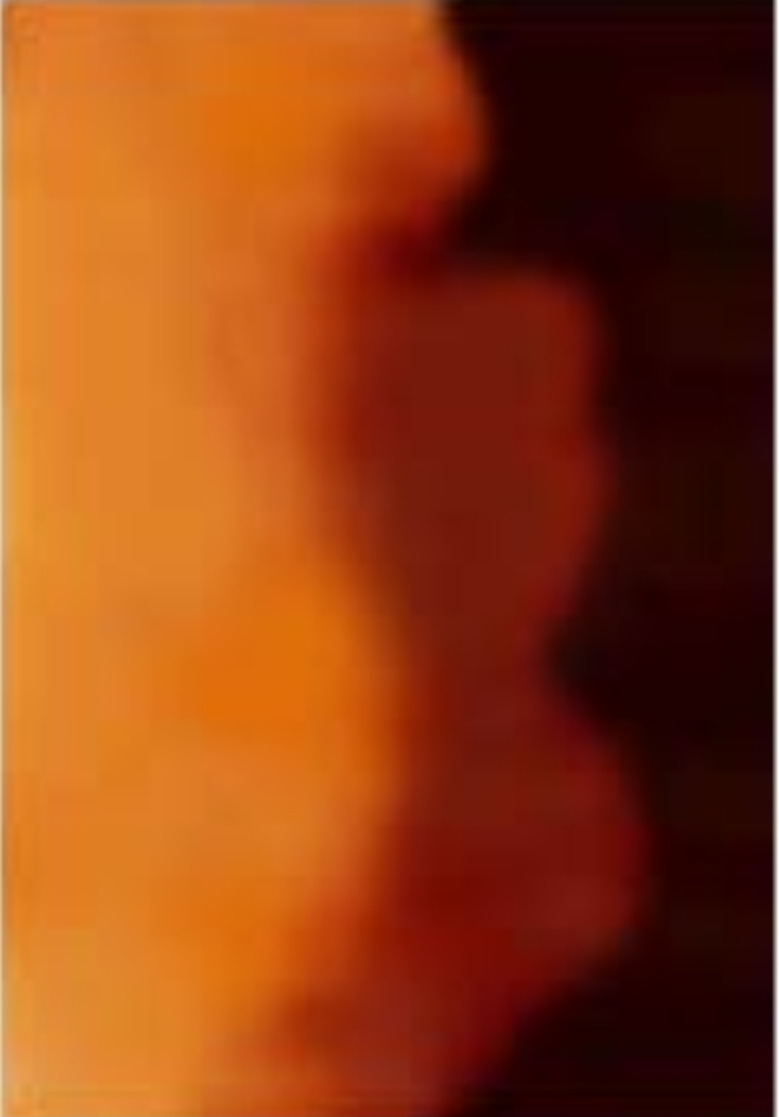
\includegraphics[width = 2.6cm]{graphene.png}
\hspace{0.65cm}
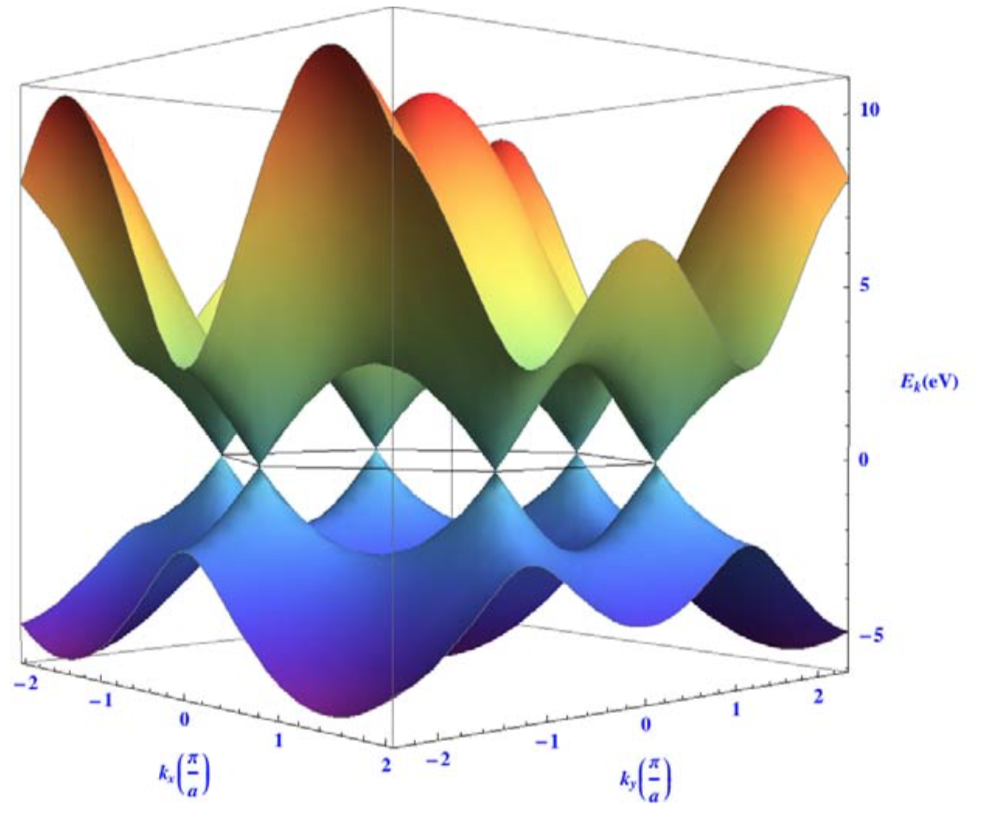
\includegraphics[width =4.5 cm]{disp_rel.png}
\caption{Left: AFM picture of a graphene monolayer. The black area is a substrate used for fabrication purposes. The dark orange area is a monolayer of graphene. Right: Dispersion relation of graphene. The black line represents the Fermi energy. Close to it, the dispersion relation is linear, corresponding to massless excitations (taken from \cite{graphene_nobel}). \label{fig:graphene}}
\end{figure}	

On the other hand, transition metal dichalcogenides (TMD's) are a recent member of the 2D materials family \cite{tmd_family1, tmd_family2, tmd_family3}. TMD's have been attracting interest because they seem to overcome some of the drawbacks of graphene in technological applications. For example, monolayer graphene is gapless, while its bilayer counterpart has only a tunable, but small gap of the order of a tenth of an $eV$. Contrastingly, TMD's have an intrinsic gap in excess of $1 \, eV$, being more promising in designing, for example, transistors. Hole-doped TMD's are expected to show topological superconductivity \cite{topological}, while the superconducting phase of graphene has been predicted, but is not easily attained. Superconductivity in graphene-like 2D materials is important because it could boost high speed nanoelectronics. Moreover, the presence of transition metal atoms in TMD's suggests the possibility of magnetic ordering \cite{tmd_magnetism}, which could be very relevant in nanospintronics applications. Both topological superconductivity and magnetic ordering arise due to the effect of strong electron correlations. Thus, to investigate these properties of TMD's when performing simulations, we need a computational method that is robust enough to capture the effects of electron interactions.\par

A nanoribbon consists of a 2D layer that can be regarded as infinitely long on one direction, but not on the other (Figure \ref{fig:fabrication}), so that edge states become relevant, and can be controlled to yield interesting properties. For simulation purposes, it is natural to assume translational invariance along the ribbon's longitudinal direction, and use periodic boundary conditions. On the other direction, we use open boundary conditions, effectively considering zigzag edges (Figure \ref{fig:nanoribbons}, left).

\begin{figure}
\centering
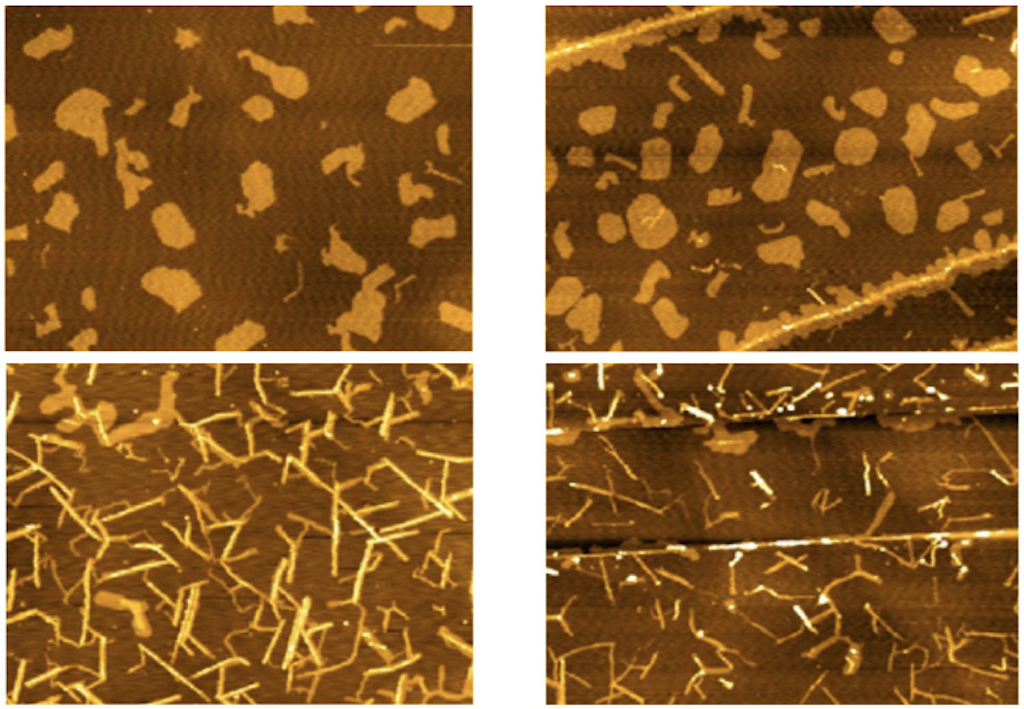
\includegraphics[scale = 0.18]{fabrication.png}
\caption{Fabrication of TMD nanoribbons. From left to right, we see AFM images showing the appeareance of nanostructures ranging from 2D nanoislands to nanoribbons, as the temperature of the substrate is increased. The nanoribbons are grown by taking advantage of the temperature dependence of shape transformations occuring during the nonequilibrium growth of this kind of surface-based nanostructures. (taken from \cite{chen}) \label{fig:fabrication}}
\end{figure}
   
A high density of low-energy electronic states is localized at the zigzag edges, decaying quickly in the bulk, which suggests the possibility of magnetic ordering. In fact, a mean field solution of the Hubbard model shows that magnetic moments are localized at the edges \cite{yazyev} (Figure \ref{fig:nanoribbons}, right). QMC has been used to investigate edge-state magnetism beyond mean field in graphene \cite{qmc_results1, qmc_results2, qmc_results3, qmc_results4, qmc_results5}. However, edge magnetism in TMD nanoribbons remains unexplored \cite{nanoribbon}.
 
\begin{figure}[ht!]
\begin{minipage}[c]{0.1\textwidth}
\centering
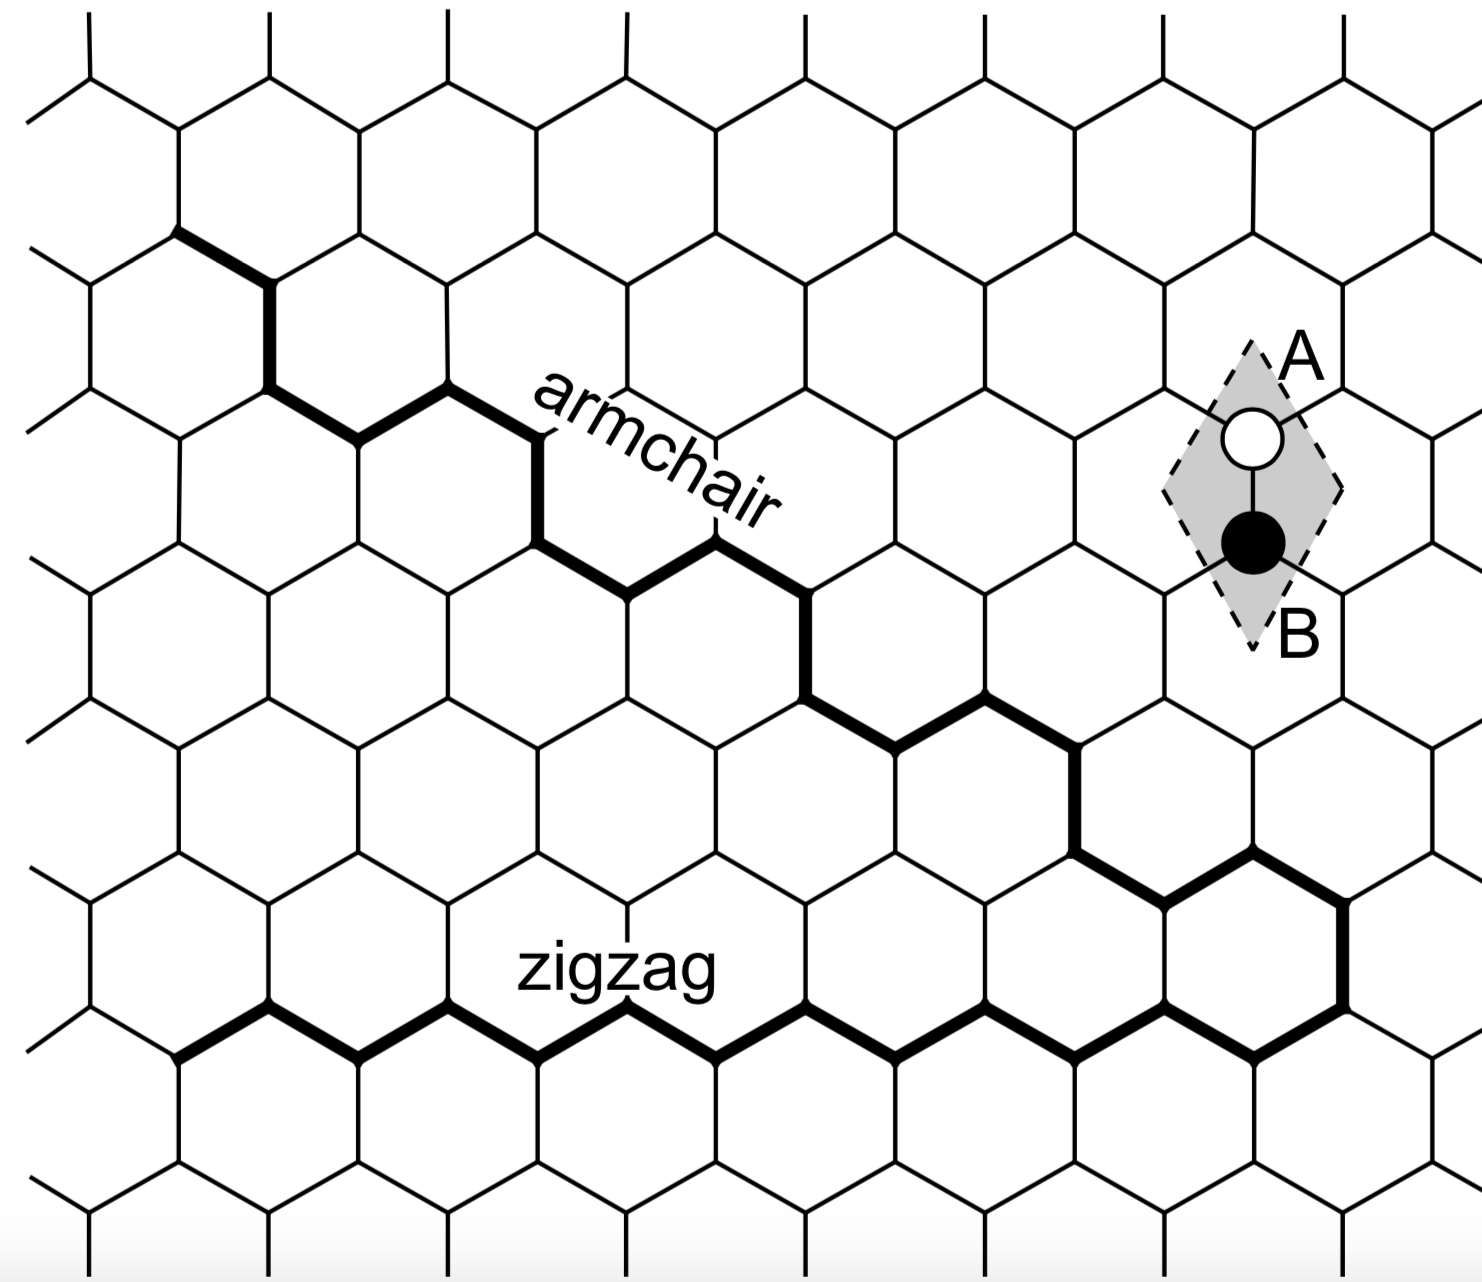
\includegraphics[scale = 0.17]{zigzag}
\end{minipage} \hspace{3cm}
\begin{minipage}[c]{0.1\textwidth}
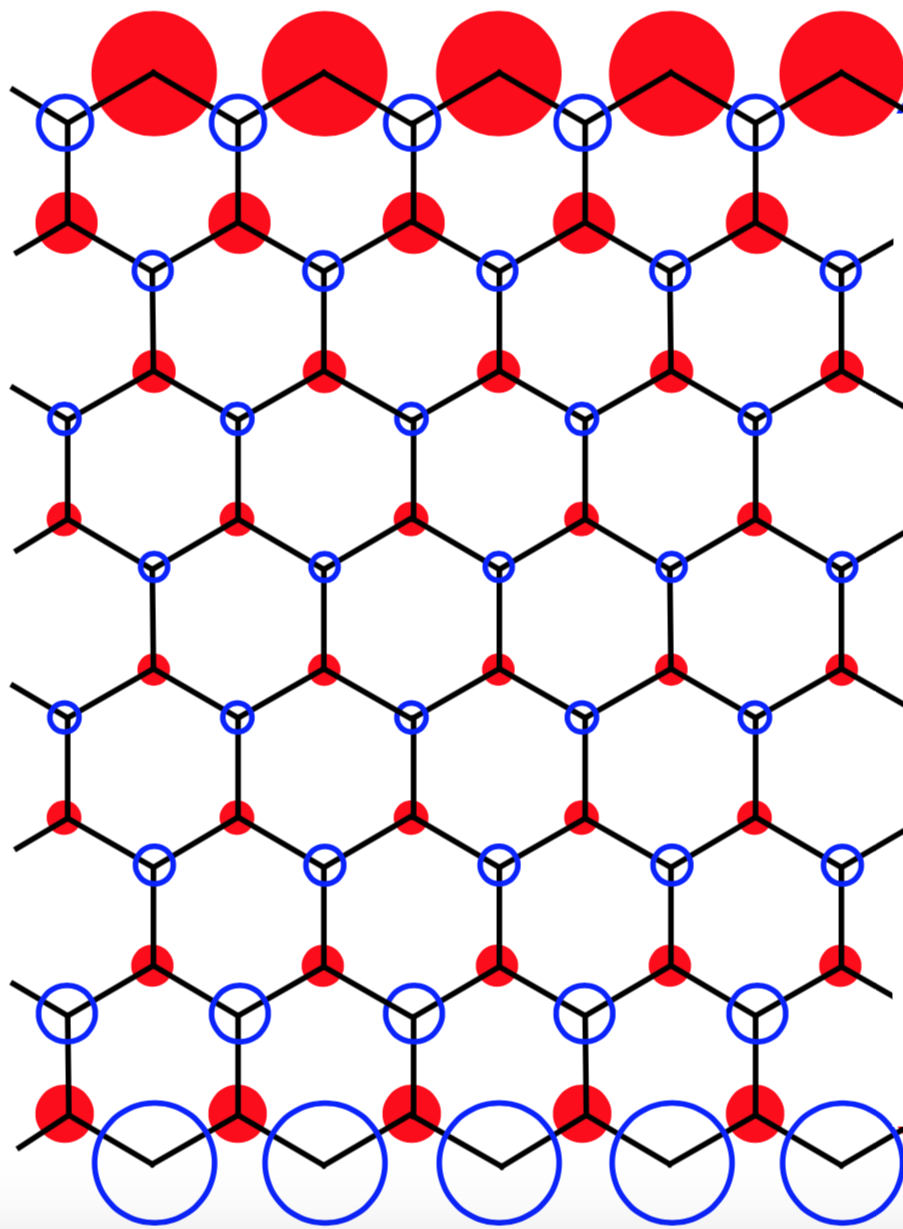
\includegraphics[scale = 0.18]{edge_states}
\end{minipage}
 \caption{Left: Two possible terminations of a TMD nanoribbon condensing in a honeycomb lattice. Right: Local magnetic moments exist on the zig zag edges. The area of the circles corresponds to the magnitude of the magnetic moment, while the color red corresponds to a spin up density, and blue to a spin down density. The accumulation of $e^-$ edge states leads to an AF ground state (opposite edges with opposite magnetic moment). (taken from \cite{yazyev}) \label{fig:nanoribbons}}
\end{figure}

While the zigzag graphene nanoribbon antiferromagnetic ground state is semiconducting, a state with interedge ferromagnetic orientation is a metal. An example of an application based on the switching between the two states is a magnetorresistive sensor. This device allows switching between low and high-resistance configurations, corresponding, respectively, to parallel, and antiparallel configurations of ferromagnetic leads at the ends of a nanoribbon. An important application of this project is precisely the investigation of the possibility of edge magnetism, as is observed in graphene nanoribbons, for TMD nanoribbons, which could yield similarly innovative applications.


\subsection*{Quantum Monte Carlo}

A variety of quantum Monte Carlo methods exists, using a sampling scheme based on the Metropolis algorithm. However, as we will see, applying them to many-fermion systems implies overcoming a significant obstacle - the so called \emph{fermion-sign problem}. The antisymmetric structure of the wave function, originating from Pauli's exclusion principle, imposes that whenever we cross a node of the wave function, there is a sign change that is at the heart of this problem. A straightforward weight interpretation of the wave function is not possible, and it is not easy to design a stochastic process driving the system to its ground state.\par

We shall also see that the \emph{fermion-sign problem} has NP \footnote{NP or nondeterministic polynomial time roughly meaning that one can devise an algorithm that verifies the "yes" answer to a decision problem in polynomial time in the system size. Note that the class $P$ - of polynomial time algorithms - is a subclass of NP.} computational complexity. One of the greatest open questions in computer science is whether $P = NP$. Solving the \emph{fermion-sign problem} would imply a solution to this problem.\par

\medskip

In this thesis, we first aim to review the existing literature on QMC methods for fermions, then become acquainted with some of the existing libraries so as to develop a code to tackle a specific problem of interacting electrons. The second part of this work has to do with the application to TMD nanoribbons and physical interpretation of results. The last phase of this project shall then consist in performing various measurements using the built QMC code, and interpreting the results in light of the relevant literature.


\section{State of the art}


The Monte Carlo method is ubiquitous. Its central idea is to use randomness to produce accurate estimates of deterministic integrals. The term was coined by Nicolas Metropolis in 1949, first appearing in a seminal paper, in which it was described as a "statistical approach to the study of differential equations, or more generally, of integro-differential equations that occur in various branches of sciences"\cite{metropolis}. Although it was used as early as 1777 in an experiment known as Buffon's needle - where one obtains an estimate of the constant $\pi$ by repeatedly throwing  a needle randomly onto a sheet of paper with evenly spaced lines - it was crucially developed in the Los Alamos National Laboratory during World War II where the development of the first atomic bomb was completed, the primary objective of the Manhattan Project. The method is particularly useful when one wants to sample from a probability distribution in an exponentially large state space. In fact, it can in principle be used to solve any problem allowing a probabilistic formulation.\par

The law of large numbers affords an approximation to integrals which can be written as an expectation of a random variable. Upon drawing enough independent samples, the sample mean gets arbitrarily close to the integral at stake. The idea is to first make an educated choice of a Markov Chain with a prescribed stationary distribution from which we ultimately desire to sample from. After a sufficiently high number of steps, a Markov Chain Monte Carlo (MCMC) algorithm generates samples from the target distribution. Imposing some conditions on this Markov Chain, namely that it should be irreducible, aperiodic and positive recurrent, the ergodic theorem guarantees that the empirical measures of the aforementioned sampler approach the target stationary distribution.\par

Quantum Monte Carlo generally provides an accurate approximation of the solution of the quantum many-body problem. When relativistic effects are negligible, which is the case of most condensed matter systems, any physical system can be described by a many-body Schr\"odinger equation. The issue is that the many-body wave function lives in the corresponding exponentially large - in the number of particles - Hilbert space. The method described above is applied to approximate the multidimensional integrals arising upon formulating the quantum many-body problem in this space. For example, the number of microstates of a physical system whose configuration space rests on a two-dimensional lattice is exponentially large.

The idea of the quantum (classical) Monte Carlo method is to simulate the random quantum (thermal) fluctuations of the system, as it oscillates between states in a given time frame \cite{newman_barkema}. Instead of visiting these states uniformly, the algorithm applies \emph{importance sampling}: the most relevant part of the phase space is sampled more frequently, overcoming the seemingly exponential complexity of computing a sample mean numerically. Even though only a small fraction of the system's states are sampled, we obtain an accurate estimate of physical quantities of interest, namely energy, and correlation functions.\par

Before resorting to fermionic QMC, one can set up a na\"ive mean field theory in which the many body wave function is approximated by an antisymmetric function of one body wave functions. One of the drawbacks of this approach is that the effect of strong fermion correlations is not captured and convergence can be slow. Going beyond mean field theory, QMC provides algorithms for both bosonic and fermionic systems. For non-frustrated boson systems, a polynomially scaling algorithm leads to an exact solution. For a fermionic system, such as the TMD nanoribbon, the algorithm usually provides an accurate yet not exact solution, which would require exponential computing time.\par


\subsection{Variational Techniques}

It is natural to combine the Metropolis algorithm for quantum many-body systems with a variational principle. The goal is to find a variational wave function which can be optimized so that ultimately we obtain as accurate as possible an estimate of the ground state of the system \cite{tao}.\par

The parameters $\bm \alpha$ of a trial wave function $\phi(\bm r)$ are optimized according to the variational principle

\begin{equation}
E[\alpha_i] = \frac{< \phi | \mathcal{H} | \phi >}{<\phi | \phi>} \ge E_0,
\end{equation}
where $E_0$ is the ground state energy.

In fact, expanding in terms of the eigenstates of the hamiltonian $\{ \psi_n (\bm r) \}$, a complete basis set:

\begin{equation}
\phi (\bm r) = \sum_{n= 0}^{\infty} a_n \psi_n (\bm r) ,
\end{equation}
and plugging it back into the variational principle, subject to $E_n \ge E_0 ,\, n > 0$ and $<\psi_n | \psi_m> = \delta_{nm}$ we obtain

\begin{equation}
E[\alpha_i] = \frac{\sum_n a_n^2 E_n}{\sum_n a_n^2 } \ge E_0
\end{equation}

The expectation is the integral

\begin{equation}
E[\alpha_i] = \frac{\int \phi^\star (\bm r) \mathcal{H} \phi (\bm r) d\bm r}{\int | \phi (\bm r') |^2 d\bm r'} \equiv \int W(\bm r) E(\bm r) d\bm r ,
\end{equation}
where the integrand is a quantity which may be regarded as a distribution function $W(\bm r) = \frac{|\phi (\bm r)|^2}{\int |\phi(\bm r')|^2 d\bm r'}$ and a local energy of the system at configuration $\bm r$: $E(\bm r) = \frac{\mathcal{H}\phi(\bm r)}{\phi (\bm r)}$.

Given $W(\bm r)$ and $E(\bm r)$, one can in principle evaluate $E[\alpha_i]$. In practice $\phi (\bm r) $ is parametrized depending on the physical model at play, and the variational parameters $\alpha_i$ in the trial wave function are optimized by minimizing $E[\alpha_i]$.\par

The Metropolis algorithm is used to sample a set of points $\{\bm r_i\}$ from the configuration space, and the evaluation of the expectation value $E[\alpha_i]$ in each QMC step for each set of variational parameters is the equivalent of computing an average of a classical quantity at a given temperature in classical Monte Carlo. Systematically, we optimize the wave function based on the Euler-Lagrange equation

\begin{equation}
\frac{\delta E[\alpha_i]}{\delta \alpha_j} = 0
\end{equation}

An example of a thorough discussion on the systematic procedure to do this is given in \cite{umrigar}.\par

An important aspect of the variational wave function - hopefully an already  reasonable approximation of the ground state - is that it should be stable when two particles approach each other and the interaction diverges. This divergence is commonly canceled by their relative kinetic energy when their separation goes to zero - \emph{cusp condition}\cite{mahan}. Building this condition into the variational wave function significantly reduces fluctuations in the results, yielding larger accuracy when dealing with systems with a larger number of particles.


\subsection{Diffusion Monte Carlo}\label{subsec:dmc}

Variational Monte Carlo is limited by the use of a trial wave function $\phi (\bm r)$: we may not have enough information to even construct a reliable variational wave function in the first place. \cite{tao}\par

Diffusion QMC allows the simulation of a many-body system while having only a limited knowledge of the system's physical properties. While it is exact for many-boson systems, it is only approximate for many-fermion systems. The idea is to map the Schr\"odinger equation into  an imaginary-time diffusion equation. Excited states are then filtered out by a diffusion process as time passes. In imaginary-time $\tau = - i t$, the solution to Schr\"odinger's equation in terms of a formal series expansion in the eigenfunctions of the hamiltonian becomes a series of transients $e^{-E_n \tau}, \, n \in \mathbb{N}$. The longest lasting of these is the ground state. \cite{kosztin} \par

The idea of DQMC is to generate samples using the exact ground state wave function $\phi_0 (\bm r)$ \cite{vmc}. The associated exact energy $E_0$ is the matrix element of the hamiltonian calculated using a trial wave function and the ground state wave function.

\begin{equation}
\begin{split}
&E_0 = \frac{ < \phi_0 |E_0 \mathbbm{1} | \phi >}{< \phi_0 | \phi >} = \\
&= \frac{< \phi_0 | \mathcal{H} | \phi >}{ <\phi_0 | \phi >} = \frac{\int d\bm r \phi_0^\star (\bm r) \phi (\bm r) E_L (\bm r)}{\int d\bm r\phi_0^\star (\bm r) \phi (\bm r)}
\end{split}
\end{equation}

Note that using this trick we avoid the computation of $\mathcal{H} \phi_0 = E_0 \phi_0$, that is, the ground state energy. Instead, we approximate the integral by considering $N$ configuration samples $\bm r_{k = 1,..., N}$ in a similar spirit to that of VQMC. Notice that the integral consists of a local energy of the trial wave function $E_L (\bm r) = \frac{\mathcal{H} \phi (\bm r)}{\phi (\bm r)}$ averaged over a mixed distribution from which we draw a sample of points $\bm r_{k=1,...N}$.

\begin{equation}
f(\bm r) = \frac{\phi_0^\star (\bm r) \phi (\bm r) }{ \int d\bm r  \phi_0 (\bm r) \phi (\bm r)}
\end{equation}

Take a single particle in 1D. Performing a Wick rotation - effectively going to imaginary time - and shifting the energy, Schr\"odinger's equation becomes

\begin{equation}
\partial_\tau \psi = -\frac{1}{2m} \partial^2_x \psi - \bigg[ V(x) - E_T \bigg] \psi
\end{equation}

The exact ground state wave function $\phi_0$ is obtained as the longest lasting transient state in imaginary time; we are interested in the asymptotic behavior of the series expansion constituting the formal solution of Schr\"odinger's equation

\begin{equation}
\psi (x, \tau) = \sum_{n=0}^{\infty} c_n \Phi_n (x) e^{-(E_n - E_T)\tau}
\end{equation}

Imaginary time evolution is governed by

\begin{equation}\label{eq:im_ev}
\begin{split}
&| \psi (t) > = \lim_{\tau \rightarrow \infty} \sum_i e^{-(E_i - E_T) \tau} |\psi_i > <\psi_i | \psi > = \\
&= \lim_{\tau \rightarrow \infty} e^{-(E_0 - E_T)\tau} | \phi_0 >< \phi_0 | \psi > 
\end{split}
\end{equation}


If $E_T > E_0$ the wave function diverges exponentially fast: $\lim_{\tau \rightarrow \infty} \psi ( x, \tau) = \infty$. Similarly, for $E_T < E_0$ it vanishes exponentially fast: $
\lim_{\tau \rightarrow \infty} \psi ( x, \tau) = 0$. However, if $E_T = E_0$ the wave function converges to the ground state one up to a constant factor.

\begin{equation}\label{eq:dmc}
\lim_{\tau \rightarrow \infty} \psi ( x, \tau) = c_0 \phi_0 (x) \,\,\, \text{, or} \quad \lim_{\tau \rightarrow \infty} |\psi (\tau) > \propto | \phi_0 >
\end{equation}

DQMC makes use of equation (\ref{eq:dmc}), approximating $\phi_0(x)$ by $\psi (x, \tau)$ for sufficiently long time. The only requirement is that $\psi (x, \tau)$ and $\phi_0(x)$ overlap significantly so that $c_0$ is large enough to be numerically measurable, and we can always center a positive trial wave function in a region where $\phi_0(x)$ is large enough. This is always possible for a single particle,  but note that it might fail for a many-fermion system for which the wave function crosses a number of nodes due to its antisymmetric nature.\par

\subsection{Path Integral Formulation}\paragraph{}

In position representation, we may rewrite equation (\ref{eq:im_ev}) by noting that

\begin{equation}\label{eq:green}
\psi(\bm r_f, \tau) = \int d\bm r_i G( \bm r_f | \bm r_i ; \tau) \psi (\bm r_i) ,
\end{equation}
where we have defined the Green function $G( \bm r_f | \bm r_i ; \tau) \equiv < \bm r_f | e^{-(\mathcal{H} - E_T) \tau} | \bm r_i >$, the imaginary-time propagator. This allows for a path integral interpretation of the diffusion method. Take equation (\ref{eq:green}), multiply by $\psi (\bm r_f)$ and divide by $\psi (\bm r_i)$ to obtain the evolution equation for the mixed distribution $f(\bm r, t) = \psi (\bm r, \tau) \psi (\bm r)$:

\begin{equation}
f(\bm r_f, \tau) = \int d\bm r_i \tilde{G} ( \bm r_f | \bm r_i; \tau) \psi (\bm r_i)^2 ,
\end{equation}
where we have redefined an \emph{importance sampling} Green function $\tilde{G} (\bm r_f | \bm r_i; \tau) = \psi (\bm r_f) G(\bm r_f | \bm r_i ; \tau) \frac{1}{\psi(\bm r_i)}$. 

The mixed distribution approaches the target stationary distribution: $f(\bm r) = \lim_{t\rightarrow \infty} f(\bm r, t) \propto \phi_0(\bm r) \psi (\bm r) $

In the limit of short propagation time, the action of the $\hat T$ and $\hat V$, the kinetic and potential energy operators, does not significantly change the states acted upon separated by the short interval $t$: $| \chi (t') >$ and $|\chi (t'+t) >$. Furthermore, one can use the Trotter-Suzuki decomposition, based on the result that for a - not necessarily commuting - set of operators $\{A_i | \, i = 1,...p\}$  we can write

\begin{equation}
e^{A_1 + A_2 + ... + A_p} = \lim_{m\rightarrow \infty} ( e^{A_1/m}e^{A_2/m}...e^{A_p/m})^m
\end{equation}

In this case it allows us to rewrite $e^{-(\hat T + \hat V) t} = e^{-\hat V t/2} e^{-\hat T t} e^{-\hat V t/2} + \mathcal{O}(t^3) $. Further acting with the potential operator on the left and on the right, we find an analytical expression for the propagator.

\begin{equation}
G(\bm r_f | \bm r_i ; \tau) \approx \frac{e^{-\frac{(\bm r_f - \bm r_i)^2}{2t} -\big( \frac{V(\bm r_f) + V(\bm r_i)}{2} - E_T \big) t}}{(2\pi t)^{3N/2}} 
\end{equation}

The \emph{fermion sign problem} will shortly become apparent. The key assumption that breaks for many-fermion wave functions is that the trial wave function does not change sign so that $\psi (\bm r_f) / \psi (\bm r_i) > 0$. In the latter case, the short time \emph{importance sampling} Green function becomes

\begin{equation}
\begin{split}
\tilde{G}(\bm r_f | \bm r_i ; \tau) \approx & \frac{1}{(2\pi t)^{3N/2}} e^{-\frac{(\bm r_f - \bm r_i - \bm v(\bm r_i)t )^2}{2t}} \\
&e^{-\big( \frac{E_L(\bm r_f) + E_L(\bm r_i)}{2} - E_T \big) t} ,
\end{split}
\end{equation}
where we introduced two quantities assumed to be constant in the short time interval: the drift velocity $\bm v(\bm r) = \nabla \psi (\bm r) / \psi (\bm r)$, and the local energy $E_L (\bm r) = \psi (\bm r)^{-1} \mathcal{H} \psi (\bm r)$. This approximation implies a finite step error that vanishes in the $t \rightarrow 0$ limit. Note that this is a solution analogous to that of a diffusion process with a drift term biasing the Brownian motion in configuration space. In practice, we obtain the stationary distribution, simulating the time evolution by iterating

\begin{equation}\label{eq:it_f}
\begin{split}
f(\bm r) &= \lim_{N\rightarrow \infty} \int d\bm r_1 d\bm r_2 ... d\bm r_N \tilde{G}(\bm r| \bm r_N ;t) \\
&\tilde{G}(\bm r_N| \bm r_{N-1} ;t) ... \tilde{G}(\bm r_2| \bm r_1 ;t) \psi(\bm r_1)^2 ,
\end{split}
\end{equation}
but the time evolution of $f$ can equivalently be shown to be given by a diffusion equation (it is done in \cite{vmc_review}): $\partial_t f = -\mathcal{L}f - (E_L (\bm r) - E_T)f$, 
where we have defined the Fokker-Planck operator $\mathcal{L} = -\frac{1}{2}\nabla^2 + \nabla \cdot \bm v(\bm r)$.\par

The stochastic realization aiming at estimating the integral in equation (\ref{eq:it_f}) is slightly more cumbersome. The Green function $\tilde{G}(\bm r_f| \bm r_i ;t)$ is not a stochastic matrix. Probability density normalization is not preserved: $\int d\bm r_f \tilde{G} ( \bm r_f | \bm r_i ; t) \neq 1$.

However, it may be written as the product of a stochastic matrix $P$ and a weight matrix $W$: $P(\bm r_f | \bm r_i) W ( \bm r_f | \bm r_i )$.

\begin{equation}
\begin{split}
P(\bm r_f | \bm r_i) &= (2\pi t)^{\frac{-3N}{2}} \exp{\bigg[-(\bm r_f -\bm r_i - \bm v(\bm r_i)t )^2 / 2t \bigg]} \\
W ( \bm r_f | \bm r_i ) &= \exp{\bigg[ \big[ (\, E_L (\bm r_f) + E_L (\bm r_i) \, )/2 - E_T \big] t \bigg]} , \\
\end{split}
\end{equation}
corresponding to a \emph{weighted random walk}. In GFQMC, one further reformulates the diffusion process so that no systematic errors due to the finite time interval $t$ arise. At each iteration $k$, a population of $M_k$ walkers at $\bm r_{k, \alpha}$ with weights $w_{k, \alpha}$ perform random walks with a branching or birth-death process in which the weights $w_{k, \alpha}$ vary only in a small range from walker to walker over the same iteration and from iteration to iteration. Under certain conditions, sampling from the correct distribution is ensured.

\subsection{Fixed-Node, Constrained Path QMC for Many-Fermion systems}

For many-fermion systems the condition of antisymmetry of the wave function may not in general be satisfied due to the finite sampling in position space. If the many-fermion wave function has nodes, a bosonic state of lower energy always exists. This means that the target ground state becomes a bosonic one for which $\psi_{B}(\bm r)$ can be chosen strictly positive.\par

By iteratively applying the Green function exactly, $\psi (\bm r)^2$ now converges to $\phi_0(\bm r) \psi (\bm r)$. This is because the trial wave function $\psi (\bm r) $ is antisymmetric and has zero overlap with the symmetric bosonic states. Finite sampling leads to the appearance of a growing and eventually dominating bosonic component $\psi_B$.\par

Now suppose you impose antisymmetry by eliminating bosonic states, i.e. considering all electron permutations in each walker. In this fermionic subspace, different paths between the same endpoints can contribute with opposite sign: $-\phi_0 $ is also a solution of the Schr\"odinger equation. Both are sampled with approximately equal probability for large enough iteration time and positive and negative weight contributions cancel out - another manifestation of the sign problem.\par

Two methods that modify DQMC to correct for the sign problem are the fixed-node approximation \cite{constrained2,vmc_review} and constrained path QMC \cite{constrained, constrained2}. The idea of the former is to force convergence to a wave function approximating the Fermionic ground state by fixing its nodes to be the same as those of the trial wave function \cite{vmc_review}. One repeats the procedure developed in the previous section for a formally defined hamiltonian $\mathcal{H}_{FN}$, which is simply the former hamiltonian with infinite potential barriers at the nodes of $\psi (\bm r)$. The energy associated with $\mathcal{H}_{FN}$ is an upper bound on the true ground state energy. Thus, the accuracy of this method depends on the shape of the nodal surface of the trial wave function. On the other hand, in constrained path QMC the ground state is represented by $|\phi_0 > = \sum_\chi c_\chi |\chi >$, where the Slater determinants $|\chi> $ are chosen so that $c_\chi > 0$. Note that this is not a unique decomposition. A constraint is placed on the random walks to account for the change to the Slater determinant basis. The two regions where the overlap $\left \langle \psi_T | \chi \right\rangle $ is either positive or negative, causing the sign problem, are not distinguishable. The approximation consists of breaking this symmetry so that the random walks are constrained to the region $\left \langle \psi_T | \chi \right\rangle > 0$.

\begin{figure}[ht!]
\centering
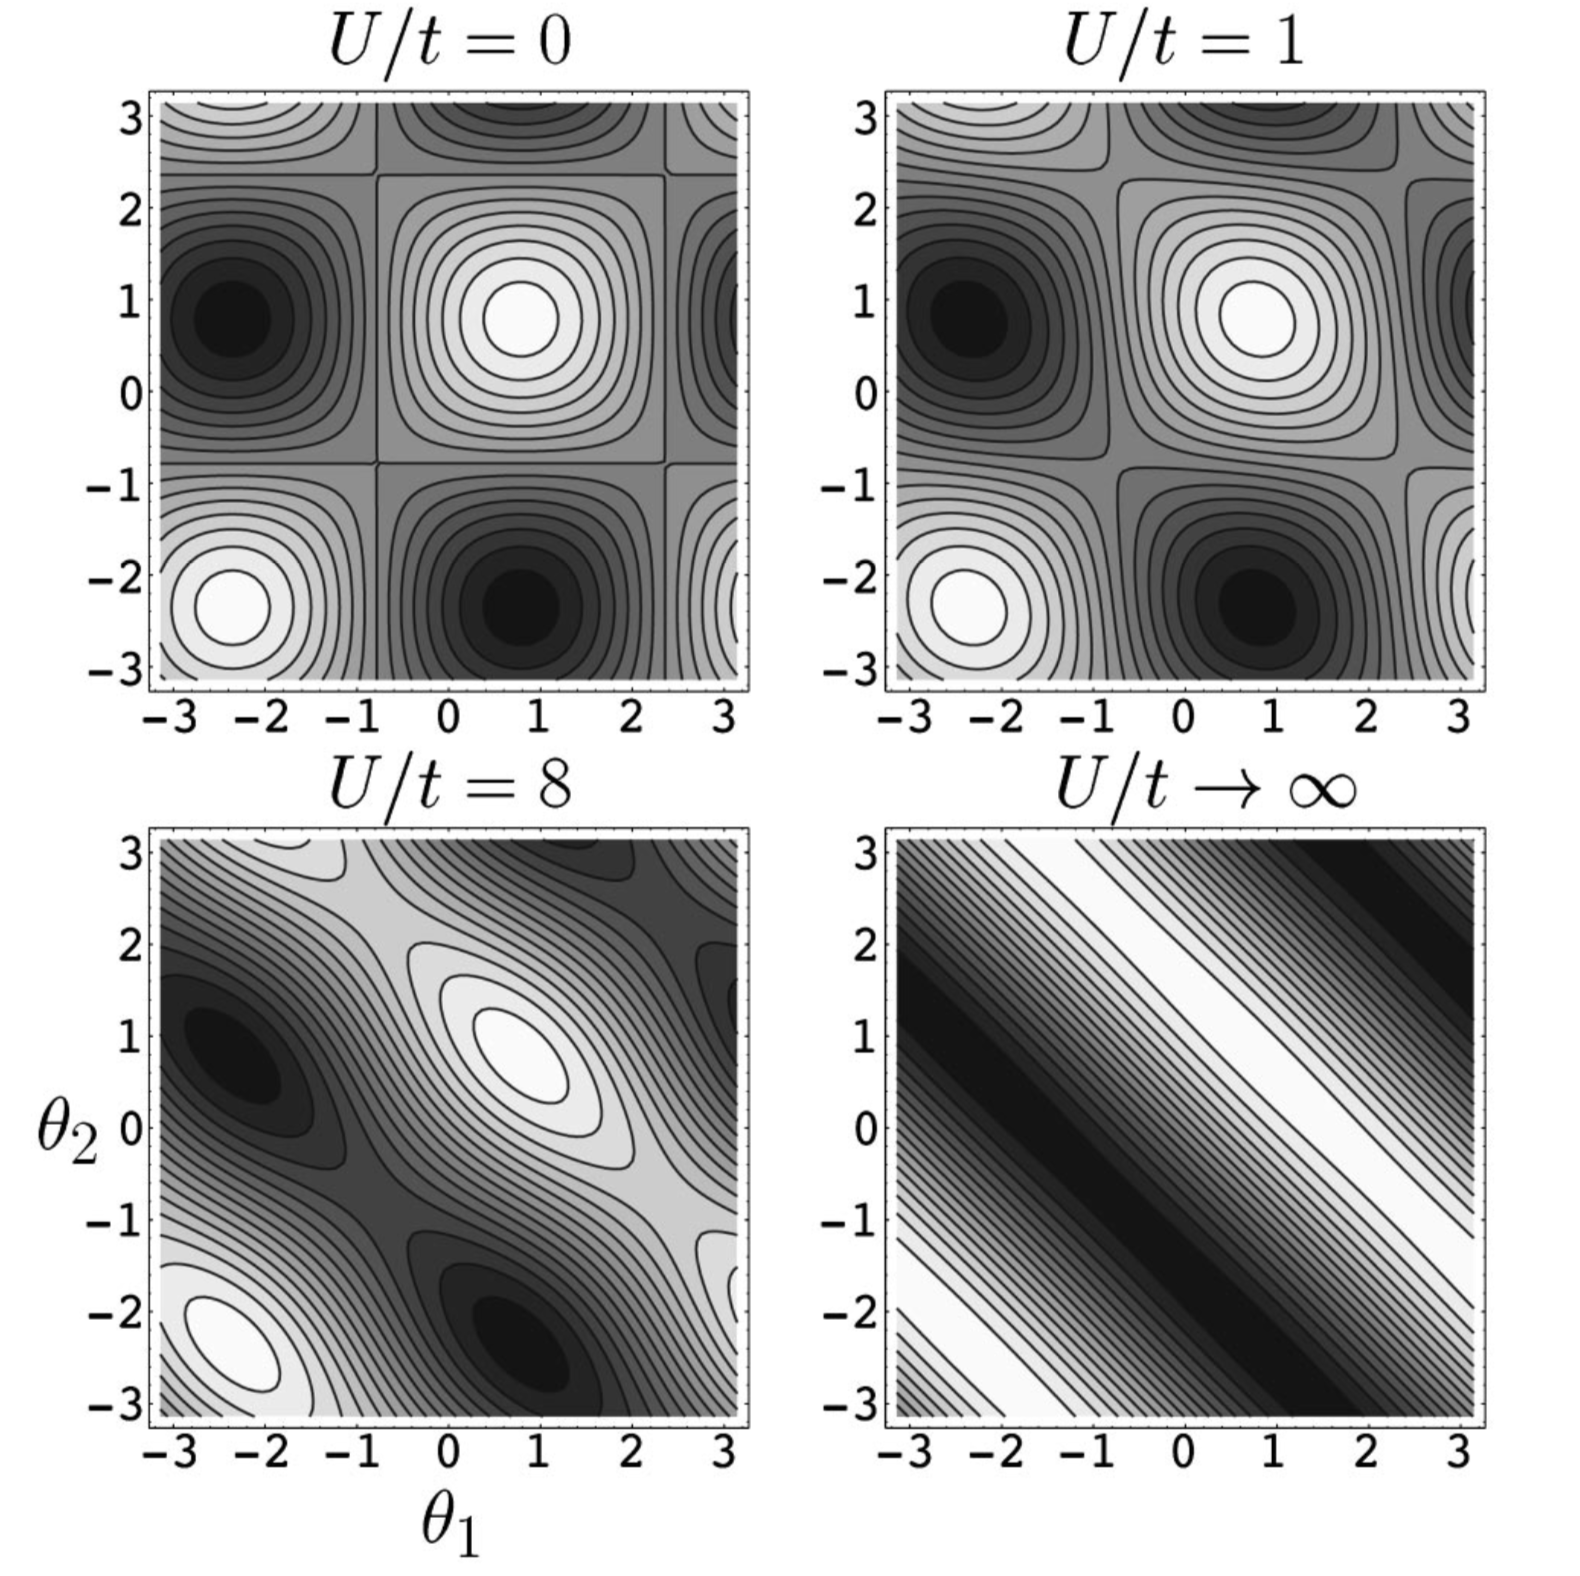
\includegraphics[width = 6cm]{constrained.png}
\caption{ Contour plots of the two-fermion ground state wave function overlap $<\chi | \phi_0 >$ for a Hubbard model as obtained in \cite{constrained2}. The parameters $\theta_{1,2}$ arise from the decomposition $|\chi > = (\cos\theta_1 c_{1\uparrow}^\dagger + \sin\theta_1 c_{2\uparrow}^\dagger) (\cos\theta_2 c_{1\downarrow}^\dagger + \sin\theta_2 c_{2\downarrow}^\dagger)$, where $c^{(\dagger)}$ are annihilation (creation) operators of two fermions with either spin up or down. Notice the varying nodal surfaces as the interaction energy-hopping parameter ratio varies. The accuracy of the constrained path QMC method depends on the shape of these surfaces (taken from \cite{constrained2}). }
\end{figure}

\subsection{Determinantal/Auxiliary Field QMC}\paragraph{}

The idea of this method is establish a mapping between quantum and classical Monte Carlo, using a suitable change of variables. The random variables are then sampled from the configuration space of the corresponding classical problem. The price to pay is that for a d-dimensional quantum problem, the corresponding classical problem is $(d+1)$-dimensional: an additional degree of freedom is added, and as we will show it corresponds to an imaginary time.

The expected value of a physical observable $\mathcal{O}$ may be written as $<\mathcal{O}> = Tr (\mathcal{O}\mathcal{P})$, where we have defined a projection operator

\begin{equation}
\mathcal{P} = \frac{1}{\mathcal{Z}}e^{-\beta\mathcal{H}} \, , \mathcal{Z} = Tr (e^{-\beta \mathcal{H}}) = \sum_i < \psi_i | e^{-\beta \mathcal{H}} | \psi_i > ,
\end{equation}
and the trace is taken over the Hilbert space describing all possible occupations in a lattice model.\par

Finding an approximation to the projection operator which is amenable to computation is done in terms of the Hubbard-Stratonovich transformation: the problem is  reformulated in terms of auxiliary variables $h_i$. The set $\{h_i\}$ is known as the Hubbard-Stratonovich field.\par

In the end, we sample configurations, that is, particular realizations of the HS field, with probability $P(h)$. It is the computation of this probability that requires determinant calculations giving the name to the method. For concreteness, we state without proof that for the example of the Hubbard model we have:

\begin{equation}
P(h) = \frac{\eta_d}{Z_h} \det [ M_{+}(h) ] \det [ M_{-}(h) ] ,
\end{equation}
where $M_\sigma (h)$ are fermion matrices depending on the imaginary time frame, spin, and the HS field; $\eta_d$ is simply a normalization constant depending on dimension, and $Z_h$ is the partition function expressed in terms of the HS field \cite{qmc}.

To move from a configuration $\{h\}$ to a new one $\{h'\}$, we vary, or flip, the value of only one variable $h_i$, leaving the rest unchanged. We use an acceptance-rejection scheme - the Metropolis-Hastings algorithm - that ensures that the accepted sample configuration follows the desired distribution. Once we reach equilibrium, i.e. the Markov Chain hits the stationary distribution, we have finished the so called warm up steps, and we may start measuring.\par

Recall the reasoning that was made in section \ref{subsec:dmc}. The solution of the Schr\"odinger equation may be expressed in terms of a linear combination of stationary states, which depend on time via a factor $e^{-iE_n t}$, where $n$ labels the energy level of the quantum system under study. We choose the energy scale so that all energies are positive and perform a change of variable to imaginary time $t= -i\tau$. The solution's time dependence is now described by a sum of transients $e^{-E_n \tau}, \, n \in \mathbb{N}$, and by following the (imaginary) time evolution of the wave function long enough, we will asymptotically reach the ground state energy $E_0$, and its corresponding wave function $\phi_0$. Note that this is independent of the initial condition in which we prepare the system. Convergence speed may eventually depend on this choice, but from a mathematical point of view if we wait long enough only the ground state will survive. The imaginary time many-body propagator $U(\tau) = e^{-H\tau}$ filters a trial wave function $\phi$ to the exact ground state $\phi_0$:

\begin{equation}
E_0 = \lim_{\tau \rightarrow \infty} \frac{<\phi | HU(\tau) | \phi >}{<\phi | U(\tau) | \phi >}
\end{equation}

We impose the condition that $\phi$ mustn't be orthogonal to $\phi_0$. Additionally, we require $\phi$ to be a symmetrized (antisymmetrized) product of single-particle orbitals for bosons (fermions).\par

The method can be used to treat systems with a variety of interactions. In general:

\begin{equation}\label{eq:general_h}
\mathcal{H} = \sum_{\alpha\beta} K_{\alpha\beta} \rho_{\beta\alpha} +\frac{1}{2} \sum_{\alpha\beta\gamma\delta} v_{\alpha\beta\gamma\delta} \rho_{\gamma\alpha} \rho_{\delta\beta} ,
\end{equation}
where $\rho_{\beta\alpha}\equiv a_\alpha^\dagger a_\beta$ and
$K_{\alpha\beta} = T_{\alpha\beta} \pm \frac{1}{2} \sum_{\gamma} v_{\alpha\gamma\gamma\beta}$
is the kinetic energy $T$ plus a self-interaction term for bosons or fermions, respectively. The subscripts ${\alpha, \beta, \gamma, \delta}$ represent eventually present degrees of freedom: spin, isospin, etc., as well as spatial coordinates \cite{sugiyama}.\par

We introduce an auxiliary field $h$ that reduces the exponential of the two-body operator in equation (\ref{eq:general_h}) to a functional integral over an infinite set of exponentials of one-body operators. We then run Monte Carlo to approximate these integrals. A valuable property of AFQMC is that it properly treats fermions: the HS representation of the propagator affords a description in terms of single-particle exactly antisymmetrized wave functions. GFQMC and DQMC do not share this property.\par

The long time behavior of a trial state: $\lim_{\tau \rightarrow \infty } e^{-\tau (\mathcal{H} - \varepsilon_0)} |\psi_T > = | \phi_0 > < \phi_0 | \psi_T >$ may be mapped onto a stochastic process in the manifold of N-particle Slater determinants $\mathcal{D}(N)$ \cite{zhang}. The mapping to a stochastic process is made possible by the discretization

\begin{equation}
e^{-\tau (\mathcal{H} - \varepsilon_0)} = (e^{-\delta \tau ( \mathcal{H} - \varepsilon_0 ) })^n \quad \text{with} \quad \delta \tau = \frac{\tau}{n}
\end{equation}

The HS transformation is in fact an operator identity that allows the establishment of a formal correspondence between a system of interacting fermions and an ensemble of non interacting fermion systems coupled to fluctuating external potentials. This leads to a random walk representation of the imaginary time evolution.\par

A limitation of the straightforward numerical implementation of AFQMC is that it leads to an exponential increase in statistical errors with imaginary time. This is due to the appearance of random complex phases during the evolution. To solve this problem, S. Zhang introduced an importance sampling transformation guiding the random walk \cite{zphase}  . This is done by introducing shift parameters in terms of which we rewrite $e^{-n\delta \tau (\mathcal{H} - \varepsilon_0)} |\psi_T >$. These parameters are chosen to minimize fluctuations in the importance function to first order in $\delta \tau$.\par

The aim is to solve the sign problem which arises when the overlap between one or more walkers and the trial state vanishes, yielding large fluctuations in the importance function, and generating statistical errors in AFQMC's estimates.

\subsection{Computational Complexity and the Sign Problem}

The sign problem afflicting many-fermion QMC causes an exponential increase of the computing time with the number of particles. A polynomially scaling algorithm would provide an unbiased and numerically exact solution (as in the case of bosons) for the problem of simulating a strongly correlated electron system. However, the problem was recently shown to be NP hard \cite{troyer}. Solving the sign problem would solve all NP problems in polynomial time (proving that $NP = P$) in what would be a major breakthrough in mathematics. This is widely believed to be unlikely, i.e. there is a conjecture that $NP \neq P$, although currently no mathematical proof exists of this impossibility.\par

Specific sign problems might be solvable. This indeed happens for a restricted subclass of quantum systems, for example see \cite{wiese, arnow,kalos}. An interesting open question is that of determining which models allow a partial solution of the sign problem due to their special properties. In particular, it is relevant for this field whether the 2D fermionic Hubbard model belongs to this class or not. A promising idea to circumvent NP hardness is to use ultracold atoms in optical lattices \cite{optical}, effectively using a quantum simulator to study the phase diagrams of correlated quantum systems. Although promising, even this method may not solve the problem in general: it is also still an open question whether a quantum computer could ever solve the NP complete problem (see \cite{troyer} and references therein).

\section{Comments on the references}
\begin{itemize}
\item \emph{Graphene and the rise of 2D materials} \cite{graphene, graphene_nobel} : review articles on the discovery of graphene and its properties. 
\item \emph{TMD nanoribbons - a new member of the 2D material family} \cite{tmd_family1, tmd_family2, tmd_family3} : reviews on the emergence of  TMD's, their electronic, magnetic, and structural properties, and prospects of future advances in nano and optoelectronics associated to the possible use of TMD's in applications.
\item \emph{Fabrication of TMD nanoribbons} \cite{chen} : discusses various experimental methods to fabricate $MoSe_2$ nanoribbons via an unusual morphological phase transition. The growth mechanism that is proposed could be applied to other TMD nanoribbons. It takes advantage of the temperature dependence of growth - the nanoribbons are obtained by increasing the temperature of a substrate - relying on shape transformations in nonequilibrium growth of surface-based nanostructures.
\item \emph{TMD nanoribbons and recent perspectives} \cite{nanoribbon,topological, tmd_magnetism} (and references therein) : recent studies in the stability of metallic edges in TMD nanoribbons, and the possibility of a superconducting phase arising in monolayer hole-doped TMD's, as well a computation of the valley/magnetic phase diagram of a monolayer hole-doped TMD, showing an instability towards an itinerant ferromagnetic phase. Valleys, i.e. degenerate valence band maxima, or conduction band minima, correspond to a degree of freedom that indicates the region of momentum space where charge carriers are confined. Carriers are then characterized not only by charge, and spin, but also by \emph{valley}, which can be used to control quantum states to generate novel devices in the framework of \emph{valleytronics}.
\item \emph{Emergence of magnetism in nanoribbons} \cite{yazyev} : this review covers the appearance of magnetic ordering in zigzag edges of graphene nanoribbons, and comments on possible applications. It also mentions some computational approaches, obtained results, and future prospects.
\item \emph{QMC results for graphene nanoribbons} \cite{qmc_results1, qmc_results2, qmc_results3, qmc_results4, qmc_results5} : Going beyond mean field, QMC has been used to investigate edge magnetism for a variety of situations in graphene, namely where strain is used to control the magnetic properties of zigzag edged nanoribbons.
\item \emph{Classical Monte Carlo} \cite{newman_barkema} : the  standard book widely used to learn the basics of classical Monte Carlo simulations in statistical physics, which are the same basic concepts used in QMC. The concepts of importance sampling, and detailed balance in the context of a Markov Chain MC are discussed.
\item \emph{Overview of aforementioned QMC methods} \cite{tao} : a recent book providing an overview of most QMC methods reviewed here. It was used throughout to learn the basic ideas of the various QMC methods.
\item \emph{A few existing QMC libraries} \cite{quest,montepython,alps,alf} : documentation of existing implementations of QMC in various programming languages.
\item \emph{Review of VQMC and DQMC} \cite{vmc_review,vmc,umrigar} : excellent review articles covering the basics of VQMC and DQMC, optimizing the trial wave functions used in VQMC. These include the concept of a variational state which is used as a starting point for QMC algorithms, and that of a diffusion Schr\"odinger equation in imaginary time. The latter is at the heart of DQMC, in the sense that all transient states, except the ground state vanish asymptotically as time goes by, which gives access to the ground state structure.
\item \emph{Path integral QMC and treating the sign problem} \cite{arnow,kosztin,constrained,constrained2, springer} : path integral formulation and improvements trying to circumvent the sign problem found in DMC. These shall be crucial in our project, once they give strategies to deal with the fermion sign problem which afflicts QMC methods applied to fermion interactions. A path integral formulation is not only of formal character. In fact, a very rich computational method arises out of it. Imposing certain conditions on the system's path in phase space allow us to control the sign problem.
\item \emph{Auxiliary Field and Phaseless Determinantal QMC} \cite{qmc,zhang,zphase} : main notes used for AFQMC and application to the Hubbard Model, phaseless AFQMC as an improved determinantal method. These articles contain the basics of determinantal QMC, and, once again, ways of combating certain numerical issues that arise in this context. 
\item \emph{The fermion sign problem is NP hard. An outlook} \cite{troyer, wiese,optical, arnow,kalos} : proof that the fermion sign problem is NP hard, models for which there is a solution to the sign problem, outlook on the future of QMC. Future perspectives on the method are presented, along with an estimate of its computational complexity. Interestingly enough, it is proved that finding a less complex QMC method for fermions would imply solving one of the most debated computer science problems we face nowadays.
\end{itemize}

\section{Work timeline}

This project will be carried out over a 20-week period. In this section we list tasks per week.
\vspace{10mm}
% #3 is yearcolumnwidth
% #4 is rulecolumnwidth
% #5 is entrycolumnwidth
% #6 is timelineheight
\begin{timeline}{1}{20}{0.5cm}{1cm}{6.5cm}{14cm}
\entry{1}{Review of Classical Monte Carlo}
\plainentry{2}{Build benchmarks for simple examples}
\entry{3}{Review of main 2D materials results and TMD's}
\entry{4}{Explore relevant QMC methods, start writing thesis}
\plainentry{5}{Review open source libraries, namely QUEST \cite{quest}, Alps \cite{alps}, Monte Python \cite{montepython}, ALF \cite{alf} }
\entry{8}{Implement QMC code, application to simple models}
\plainentry{10}{Determine which are the main quantities to measure for TMD nanoribbons}
\entry{12}{Implement measurements and test the code on more complex models}
\entry{16}{Start performing QMC measurements}
\entry{18}{Compile and interpret results}
\entry{20}{Finish writing thesis, review and editing}
\end{timeline}

\printbibliography

\end{document}
\documentclass[10pt, twocolumn, twoside]{article}
\usepackage[T1]{fontenc}
\usepackage{cuted}
\usepackage{lipsum}
\usepackage{graphicx}
\usepackage{bm}
\usepackage{geometry}
\usepackage{bbm}
\geometry{a4paper,total={170mm,257mm},left=20mm,top=20mm,}
\pagenumbering{arabic}
\usepackage{hyperref}
\usepackage{url}
\usepackage{scrextend}
\usepackage{amsmath,amssymb}
\usepackage[
backend=biber,
style=nature,
sorting=none
]{biblatex}
\addbibresource{thesis_outline.bib}

\newenvironment{alphafootnotes}
  {\par\edef\savedfootnotenumber{\number\value{footnote}}
   \renewcommand{\thefootnote}{\alph{footnote}}
   \setcounter{footnote}{0}}
  {\par\setcounter{footnote}{\savedfootnotenumber}}


\usepackage{tikz}

\usetikzlibrary{arrows, calc, decorations.markings, positioning}

\author{Francisco Monteiro de Oliveira Brito \footnotemark}
\title{Development of a QMC code to tackle interacting electronic systems in 2D with application to TMD nanoribbons  \\ \bigskip  \small{MSc Engineering Physics Thesis Outline\\ \medskip supervised by Jo\~ao M. V. P. Lopes (CFP - Centro de F\'isica do Porto) and Eduardo F. V. Castro (CeFEMA)} }
\date{\today}
\setlength\columnsep{3em}

\makeatletter
\newenvironment{timeline}[6]{%
    % #1 is startyear
    % #2 is tlendyear
    % #3 is yearcolumnwidth
    % #4 is rulecolumnwidth
    % #5 is entrycolumnwidth
    % #6 is timelineheight

    \newcommand{\startyear}{#1}
    \newcommand{\tlendyear}{#2}

    \newcommand{\yearcolumnwidth}{#3}
    \newcommand{\rulecolumnwidth}{#4}
    \newcommand{\entrycolumnwidth}{#5}
    \newcommand{\timelineheight}{#6}

    \newcommand{\templength}{}

    \newcommand{\entrycounter}{0}

    % https://tex.stackexchange.com/questions/85528/checking-whether-or-not-a-node-has-been-previously-defined
    % https://tex.stackexchange.com/questions/37709/how-can-i-know-if-a-node-is-already-defined
    \long\def\ifnodedefined##1##2##3{%
        \@ifundefined{pgf@sh@ns@##1}{##3}{##2}%
    }

    \newcommand{\ifnodeundefined}[2]{%
        \ifnodedefined{##1}{}{##2}
    }

    \newcommand{\drawtimeline}{%
        \draw[timelinerule] (\yearcolumnwidth+5pt, 0pt) -- (\yearcolumnwidth+5pt, -\timelineheight);
        \draw (\yearcolumnwidth+0pt, -10pt) -- (\yearcolumnwidth+10pt, -10pt);
        \draw (\yearcolumnwidth+0pt, -\timelineheight+15pt) -- (\yearcolumnwidth+10pt, -\timelineheight+15pt);

        \pgfmathsetlengthmacro{\templength}{neg(add(multiply(subtract(\startyear, \startyear), divide(subtract(\timelineheight, 25), subtract(\tlendyear, \startyear))), 10))}
        \node[year] (year-\startyear) at (\yearcolumnwidth, \templength) {\startyear};

        \pgfmathsetlengthmacro{\templength}{neg(add(multiply(subtract(\tlendyear, \startyear), divide(subtract(\timelineheight, 25), subtract(\tlendyear, \startyear))), 10))}
        \node[year] (year-\tlendyear) at (\yearcolumnwidth, \templength) {\tlendyear};
    }

    \newcommand{\entry}[2]{%
        % #1 is the year
        % #2 is the entry text

        \pgfmathtruncatemacro{\lastentrycount}{\entrycounter}
        \pgfmathtruncatemacro{\entrycounter}{\entrycounter + 1}

        \ifdim \lastentrycount pt > 0 pt%
            \node[entry] (entry-\entrycounter) [below of=entry-\lastentrycount] {##2};
        \else%
            \pgfmathsetlengthmacro{\templength}{neg(add(multiply(subtract(\startyear, \startyear), divide(subtract(\timelineheight, 25), subtract(\tlendyear, \startyear))), 10))}
            \node[entry] (entry-\entrycounter) at (\yearcolumnwidth+\rulecolumnwidth+10pt, \templength) {##2};
        \fi

        \ifnodeundefined{year-##1}{%
            \pgfmathsetlengthmacro{\templength}{neg(add(multiply(subtract(##1, \startyear), divide(subtract(\timelineheight, 25), subtract(\tlendyear, \startyear))), 10))}
            \draw (\yearcolumnwidth+2.5pt, \templength) -- (\yearcolumnwidth+7.5pt, \templength);
            \node[year] (year-##1) at (\yearcolumnwidth, \templength) {##1};
        }

        \draw ($(year-##1.east)+(2.5pt, 0pt)$) -- ($(year-##1.east)+(7.5pt, 0pt)$) -- ($(entry-\entrycounter.west)-(5pt,0)$) -- (entry-\entrycounter.west);
    }

    \newcommand{\plainentry}[2]{% plainentry won't print date in the timeline
        % #1 is the year
        % #2 is the entry text

        \pgfmathtruncatemacro{\lastentrycount}{\entrycounter}
        \pgfmathtruncatemacro{\entrycounter}{\entrycounter + 1}

        \ifdim \lastentrycount pt > 0 pt%
            \node[entry] (entry-\entrycounter) [below of=entry-\lastentrycount] {##2};
        \else%
            \pgfmathsetlengthmacro{\templength}{neg(add(multiply(subtract(\startyear, \startyear), divide(subtract(\timelineheight, 25), subtract(\tlendyear, \startyear))), 10))}
            \node[entry] (entry-\entrycounter) at (\yearcolumnwidth+\rulecolumnwidth+10pt, \templength) {##2};
        \fi

        \ifnodeundefined{invisible-year-##1}{%
            \pgfmathsetlengthmacro{\templength}{neg(add(multiply(subtract(##1, \startyear), divide(subtract(\timelineheight, 25), subtract(\tlendyear, \startyear))), 10))}
            \draw (\yearcolumnwidth+2.5pt, \templength) -- (\yearcolumnwidth+7.5pt, \templength);
            \node[year] (invisible-year-##1) at (\yearcolumnwidth, \templength) {};
        }

        \draw ($(invisible-year-##1.east)+(2.5pt, 0pt)$) -- ($(invisible-year-##1.east)+(7.5pt, 0pt)$) -- ($(entry-\entrycounter.west)-(5pt,0)$) -- (entry-\entrycounter.west);
    }

    \begin{tikzpicture}
        \tikzstyle{entry} = [%
            align=left,%
            text width=\entrycolumnwidth,%
            node distance=13mm,%
            anchor=west]
        \tikzstyle{year} = [anchor=east]
        \tikzstyle{timelinerule} = [%
            draw,%
            decoration={markings, mark=at position 1 with {\arrow[scale=1.5]{latex'}}},%
            postaction={decorate},%
            shorten >=0.4pt]

        \drawtimeline
}
{
    \end{tikzpicture}
    \let\startyear\@undefined
    \let\tlendyear\@undefined
    \let\yearcolumnwidth\@undefined
    \let\rulecolumnwidth\@undefined
    \let\entrycolumnwidth\@undefined
    \let\timelineheight\@undefined
    \let\entrycounter\@undefined
    \let\ifnodedefined\@undefined
    \let\ifnodeundefined\@undefined
    \let\drawtimeline\@undefined
    \let\entry\@undefined
}
\makeatother


\begin{document}
\begin{alphafootnotes}
\footnotetext{*CeFEMA - Center of Physics and Engineering of Advanced Materials, Physics Department, Instituto Superior T\'ecnico, University of Lisbon, Av. Rovisco Pais, 1049-001 Lisbon, Portugal}
\end{alphafootnotes}

%\author{Francisco Monteiro de Oliveira Brito\footnote{CeFEMA - Center of Physics and Engineering of Advanced Materials, Physics Department, Instituto Superior T\'ecnico, University of Lisbon, Av. Rovisco Pais, 1049-001 Lisbon, Portugal}}
%\title{Development of a QMC code to tackle interacting electronic systems in 2D with application to TMD nanoribbons  \\ \bigskip  \small{MSc Engineering Physics Thesis Outline\\ \medskip supervised by Jo\~ao M. V. P. Lopes (CFP - Centro de F\'isica do Porto) and Eduardo F. V. Castro (CeFEMA)} }
%\maketitle

\begin{strip}
  \vspace*{\dimexpr-\baselineskip-\stripsep\relax}
  \centering
  \maketitle
  \vskip\baselineskip
\noindent\makebox[\textwidth]{\rule{1.1\paperwidth}{0.4pt}}
  \vskip\baselineskip
\end{strip}

\begin{abstract}
The isolation of graphene in 2004 has led to a growing interest of the scientific community in two-dimensional materials revealing extraordinary properties.  In fact, their very existence was not expected \emph{a priori} because at first sight they seem to violate the Mermin-Wagner theorem. A vast set of open problems remains to be solved within the realm of their fascinating and counterintuitive properties. These are often tackled by carrying out numerical simulations. Quantum Monte Carlo (QMC) is a simulation method that is amply applicable to condensed matter physics problems. Despite the system size being constrained due to limited simulation time, reliable and accurate solutions are provided to the otherwise intractable quantum many-body problem. The field is currently very active and method optimization can prove crucial in applications to real physical systems. We will use QMC to simulate a two-dimensional system with strong electron interactions giving rise to promising properties: a nanostructure made of a recent member of the 2D materials family called a nanoribbon.
\end{abstract}


\section{Introduction and aim}

Solving the many-body problem remains one of the greatest challenges in physics. Following the wealth of attempts at such pursuit, certain phenomena arising due to the strong interactions in quantum systems are explained in different theoretical frameworks, namely conventional superconductivity, the Mott metal-insulator transition, and fractional quantum Hall effect. All of these breakthroughs represented revolutions in their respective fields with both a scientific and technological impact.\par

Only in very limited cases does an analytical solution exist for the problem of solving the Schr\"odinger equation for a system of many strongly interacting particles\footnote{A few solvable models exist, for example the 1D Hubbard model via Bethe \emph{ansatz}.}. Different approximations provide information about the role played by the competing interactions under various conditions. It is then natural that numerical methods have become prominent as a tool for extracting useful information about this type of systems. QMC is amongst the most accurate and extensively studied ones.\par


\subsection*{Beyond graphene: TMD nanoribbons}

Two-dimensional materials have steadily been attracting the interest of the scientific community since 2004, when graphene was experimentally isolated from a 3D graphite base, yielding a system constituted by a single layer of atoms (Figure \ref{fig:graphene}, left).
Since then, numerous studies have been made due to the promising properties of these materials, and the interesting as-yet-unseen phenomena occurring within them, for example: unconventional quantum Hall effect, absence of localization, and electrons behaving like massless relativistic particles (Figure \ref{fig:graphene}, right), providing a bridge between condensed matter physics and quantum electrodynamics \cite{graphene}.

\begin{figure}[ht!]
\centering
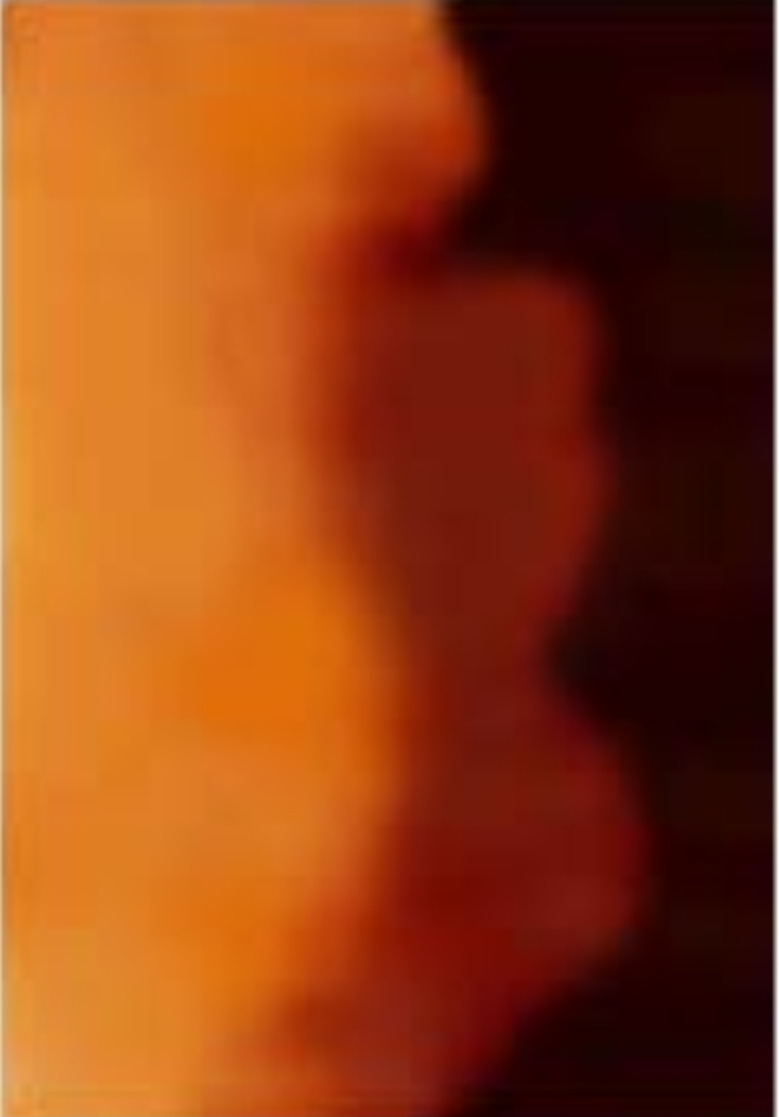
\includegraphics[width = 2.6cm]{graphene.png}
\hspace{0.65cm}
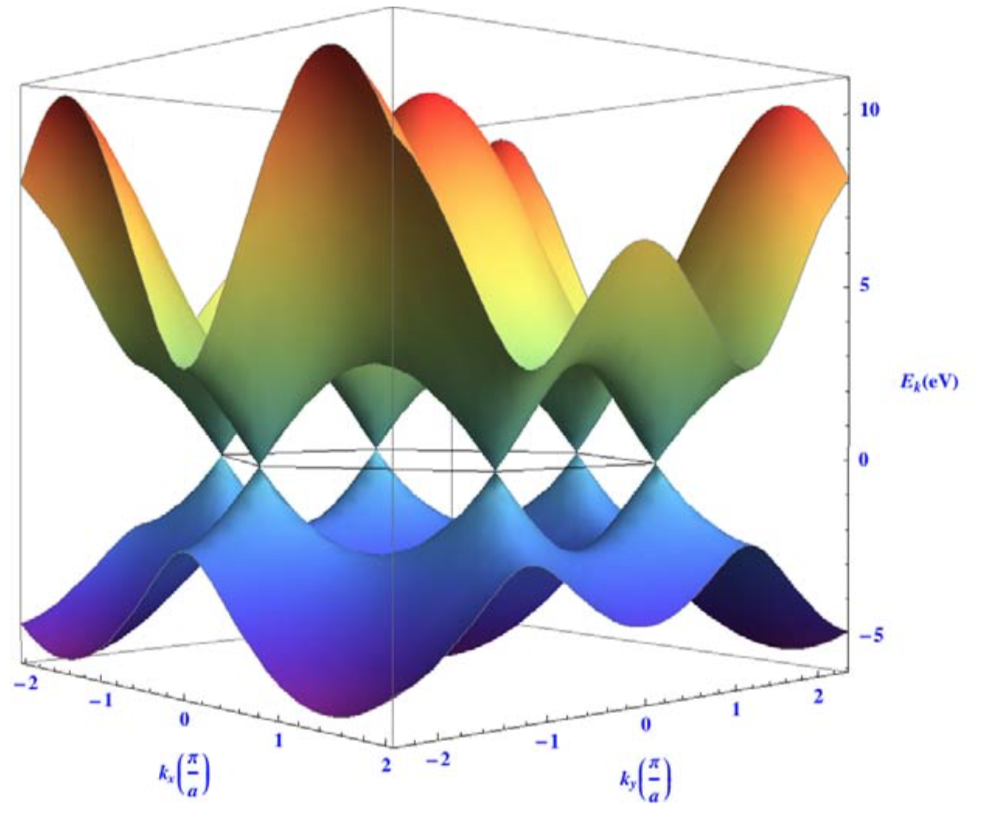
\includegraphics[width =4.5 cm]{disp_rel.png}
\caption{Left: AFM picture of a graphene monolayer. The black area is a substrate used for fabrication purposes. The dark orange area is a monolayer of graphene. Right: Dispersion relation of graphene. The black line represents the Fermi energy. Close to it, the dispersion relation is linear, corresponding to massless excitations (taken from \cite{graphene_nobel}). \label{fig:graphene}}
\end{figure}	

On the other hand, transition metal dichalcogenides (TMD's) are a recent member of the 2D materials family \cite{tmd_family1, tmd_family2, tmd_family3}. TMD's have been attracting interest because they seem to overcome some of the drawbacks of graphene in technological applications. For example, monolayer graphene is gapless, while its bilayer counterpart has only a tunable, but small gap of the order of a tenth of an $eV$. Contrastingly, TMD's have an intrinsic gap in excess of $1 \, eV$, being more promising in designing, for example, transistors. Hole-doped TMD's are expected to show topological superconductivity \cite{topological}, while the superconducting phase of graphene has been predicted, but is not easily attained. Superconductivity in graphene-like 2D materials is important because it could boost high speed nanoelectronics. Moreover, the presence of transition metal atoms in TMD's suggests the possibility of magnetic ordering \cite{tmd_magnetism}, which could be very relevant in nanospintronics applications. Both topological superconductivity and magnetic ordering arise due to the effect of strong electron correlations. Thus, to investigate these properties of TMD's when performing simulations, we need a computational method that is robust enough to capture the effects of electron interactions.\par

A nanoribbon consists of a 2D layer that can be regarded as infinitely long on one direction, but not on the other (Figure \ref{fig:fabrication}), so that edge states become relevant, and can be controlled to yield interesting properties. For simulation purposes, it is natural to assume translational invariance along the ribbon's longitudinal direction, and use periodic boundary conditions. On the other direction, we use open boundary conditions, effectively considering zigzag edges (Figure \ref{fig:nanoribbons}, left).

\begin{figure}
\centering
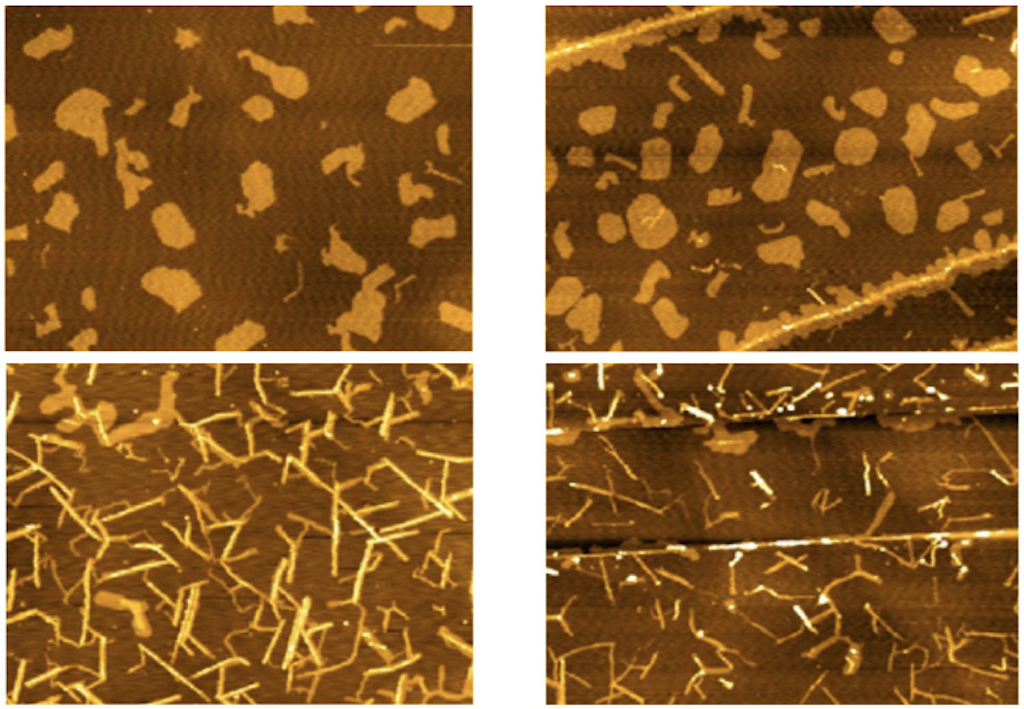
\includegraphics[scale = 0.18]{fabrication.png}
\caption{Fabrication of TMD nanoribbons. From left to right, we see AFM images showing the appeareance of nanostructures ranging from 2D nanoislands to nanoribbons, as the temperature of the substrate is increased. The nanoribbons are grown by taking advantage of the temperature dependence of shape transformations occuring during the nonequilibrium growth of this kind of surface-based nanostructures. (taken from \cite{chen}) \label{fig:fabrication}}
\end{figure}
   
A high density of low-energy electronic states is localized at the zigzag edges, decaying quickly in the bulk, which suggests the possibility of magnetic ordering. In fact, a mean field solution of the Hubbard model shows that magnetic moments are localized at the edges \cite{yazyev} (Figure \ref{fig:nanoribbons}, right). QMC has been used to investigate edge-state magnetism beyond mean field in graphene \cite{qmc_results1, qmc_results2, qmc_results3, qmc_results4, qmc_results5}. However, edge magnetism in TMD nanoribbons remains unexplored \cite{nanoribbon}.
 
\begin{figure}[ht!]
\begin{minipage}[c]{0.1\textwidth}
\centering
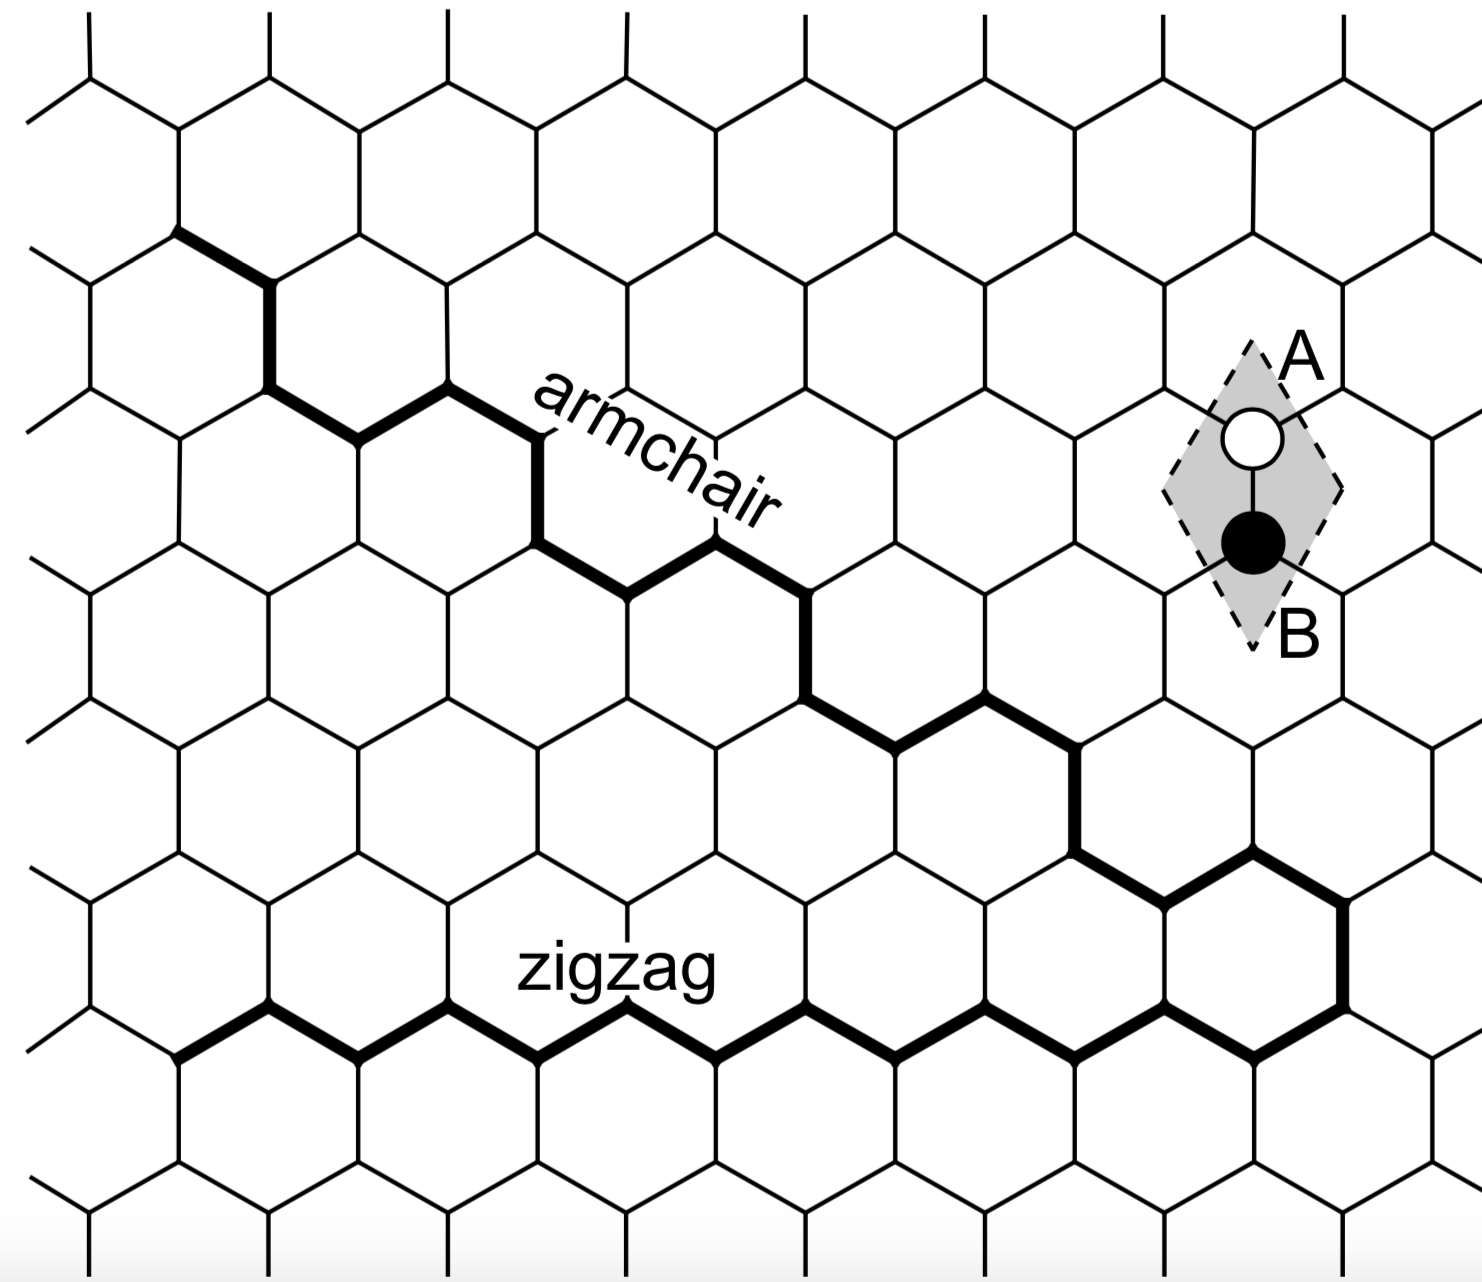
\includegraphics[scale = 0.17]{zigzag}
\end{minipage} \hspace{3cm}
\begin{minipage}[c]{0.1\textwidth}
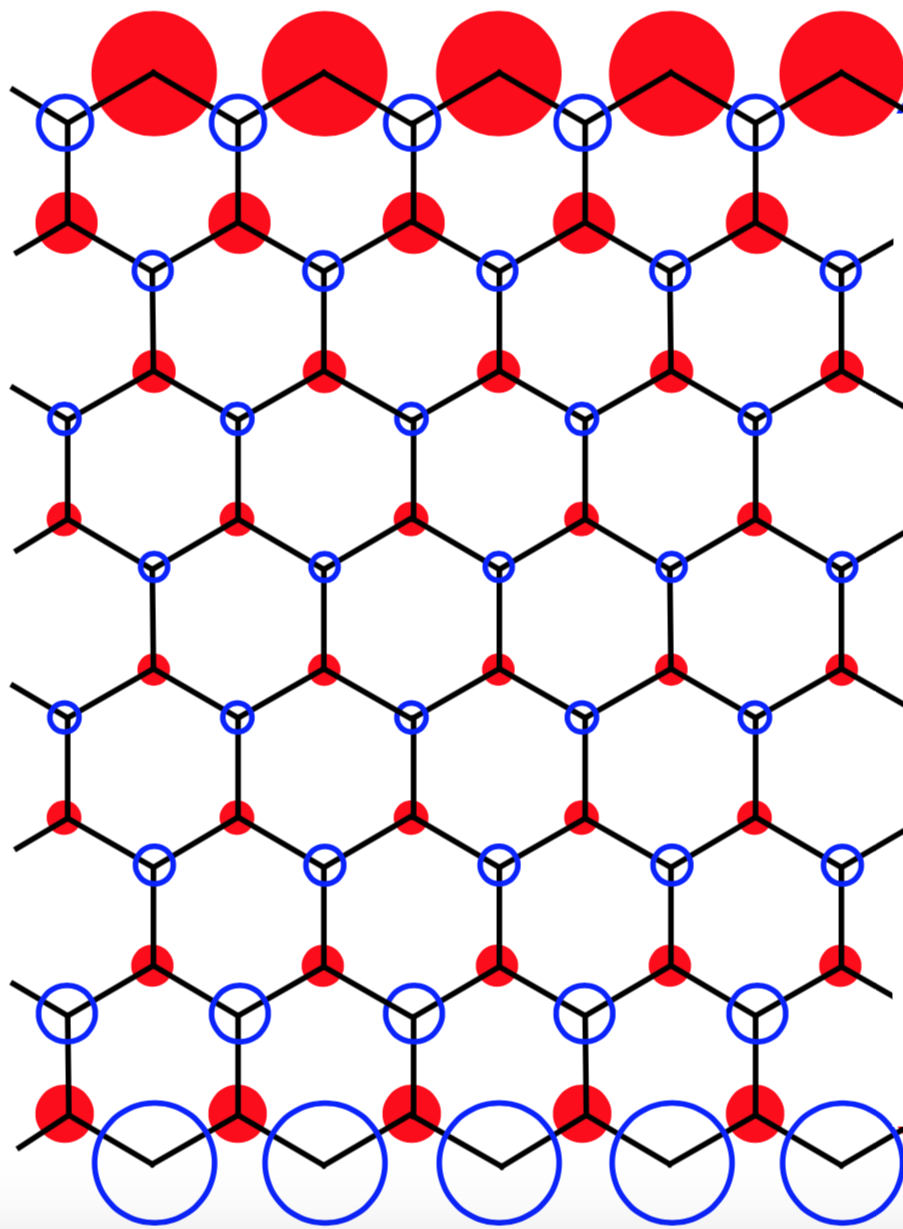
\includegraphics[scale = 0.18]{edge_states}
\end{minipage}
 \caption{Left: Two possible terminations of a TMD nanoribbon condensing in a honeycomb lattice. Right: Local magnetic moments exist on the zig zag edges. The area of the circles corresponds to the magnitude of the magnetic moment, while the color red corresponds to a spin up density, and blue to a spin down density. The accumulation of $e^-$ edge states leads to an AF ground state (opposite edges with opposite magnetic moment). (taken from \cite{yazyev}) \label{fig:nanoribbons}}
\end{figure}

While the zigzag graphene nanoribbon antiferromagnetic ground state is semiconducting, a state with interedge ferromagnetic orientation is a metal. An example of an application based on the switching between the two states is a magnetorresistive sensor. This device allows switching between low and high-resistance configurations, corresponding, respectively, to parallel, and antiparallel configurations of ferromagnetic leads at the ends of a nanoribbon. An important application of this project is precisely the investigation of the possibility of edge magnetism, as is observed in graphene nanoribbons, for TMD nanoribbons, which could yield similarly innovative applications.


\subsection*{Quantum Monte Carlo}

A variety of quantum Monte Carlo methods exists, using a sampling scheme based on the Metropolis algorithm. However, as we will see, applying them to many-fermion systems implies overcoming a significant obstacle - the so called \emph{fermion-sign problem}. The antisymmetric structure of the wave function, originating from Pauli's exclusion principle, imposes that whenever we cross a node of the wave function, there is a sign change that is at the heart of this problem. A straightforward weight interpretation of the wave function is not possible, and it is not easy to design a stochastic process driving the system to its ground state.\par

We shall also see that the \emph{fermion-sign problem} has NP \footnote{NP or nondeterministic polynomial time roughly meaning that one can devise an algorithm that verifies the "yes" answer to a decision problem in polynomial time in the system size. Note that the class $P$ - of polynomial time algorithms - is a subclass of NP.} computational complexity. One of the greatest open questions in computer science is whether $P = NP$. Solving the \emph{fermion-sign problem} would imply a solution to this problem.\par

\medskip

In this thesis, we first aim to review the existing literature on QMC methods for fermions, then become acquainted with some of the existing libraries so as to develop a code to tackle a specific problem of interacting electrons. The second part of this work has to do with the application to TMD nanoribbons and physical interpretation of results. The last phase of this project shall then consist in performing various measurements using the built QMC code, and interpreting the results in light of the relevant literature.


\section{State of the art}


The Monte Carlo method is ubiquitous. Its central idea is to use randomness to produce accurate estimates of deterministic integrals. The term was coined by Nicolas Metropolis in 1949, first appearing in a seminal paper, in which it was described as a "statistical approach to the study of differential equations, or more generally, of integro-differential equations that occur in various branches of sciences"\cite{metropolis}. Although it was used as early as 1777 in an experiment known as Buffon's needle - where one obtains an estimate of the constant $\pi$ by repeatedly throwing  a needle randomly onto a sheet of paper with evenly spaced lines - it was crucially developed in the Los Alamos National Laboratory during World War II where the development of the first atomic bomb was completed, the primary objective of the Manhattan Project. The method is particularly useful when one wants to sample from a probability distribution in an exponentially large state space. In fact, it can in principle be used to solve any problem allowing a probabilistic formulation.\par

The law of large numbers affords an approximation to integrals which can be written as an expectation of a random variable. Upon drawing enough independent samples, the sample mean gets arbitrarily close to the integral at stake. The idea is to first make an educated choice of a Markov Chain with a prescribed stationary distribution from which we ultimately desire to sample from. After a sufficiently high number of steps, a Markov Chain Monte Carlo (MCMC) algorithm generates samples from the target distribution. Imposing some conditions on this Markov Chain, namely that it should be irreducible, aperiodic and positive recurrent, the ergodic theorem guarantees that the empirical measures of the aforementioned sampler approach the target stationary distribution.\par

Quantum Monte Carlo generally provides an accurate approximation of the solution of the quantum many-body problem. When relativistic effects are negligible, which is the case of most condensed matter systems, any physical system can be described by a many-body Schr\"odinger equation. The issue is that the many-body wave function lives in the corresponding exponentially large - in the number of particles - Hilbert space. The method described above is applied to approximate the multidimensional integrals arising upon formulating the quantum many-body problem in this space. For example, the number of microstates of a physical system whose configuration space rests on a two-dimensional lattice is exponentially large.

The idea of the quantum (classical) Monte Carlo method is to simulate the random quantum (thermal) fluctuations of the system, as it oscillates between states in a given time frame \cite{newman_barkema}. Instead of visiting these states uniformly, the algorithm applies \emph{importance sampling}: the most relevant part of the phase space is sampled more frequently, overcoming the seemingly exponential complexity of computing a sample mean numerically. Even though only a small fraction of the system's states are sampled, we obtain an accurate estimate of physical quantities of interest, namely energy, and correlation functions.\par

Before resorting to fermionic QMC, one can set up a na\"ive mean field theory in which the many body wave function is approximated by an antisymmetric function of one body wave functions. One of the drawbacks of this approach is that the effect of strong fermion correlations is not captured and convergence can be slow. Going beyond mean field theory, QMC provides algorithms for both bosonic and fermionic systems. For non-frustrated boson systems, a polynomially scaling algorithm leads to an exact solution. For a fermionic system, such as the TMD nanoribbon, the algorithm usually provides an accurate yet not exact solution, which would require exponential computing time.\par


\subsection{Variational Techniques}

It is natural to combine the Metropolis algorithm for quantum many-body systems with a variational principle. The goal is to find a variational wave function which can be optimized so that ultimately we obtain as accurate as possible an estimate of the ground state of the system \cite{tao}.\par

The parameters $\bm \alpha$ of a trial wave function $\phi(\bm r)$ are optimized according to the variational principle

\begin{equation}
E[\alpha_i] = \frac{< \phi | \mathcal{H} | \phi >}{<\phi | \phi>} \ge E_0,
\end{equation}
where $E_0$ is the ground state energy.

In fact, expanding in terms of the eigenstates of the hamiltonian $\{ \psi_n (\bm r) \}$, a complete basis set:

\begin{equation}
\phi (\bm r) = \sum_{n= 0}^{\infty} a_n \psi_n (\bm r) ,
\end{equation}
and plugging it back into the variational principle, subject to $E_n \ge E_0 ,\, n > 0$ and $<\psi_n | \psi_m> = \delta_{nm}$ we obtain

\begin{equation}
E[\alpha_i] = \frac{\sum_n a_n^2 E_n}{\sum_n a_n^2 } \ge E_0
\end{equation}

The expectation is the integral

\begin{equation}
E[\alpha_i] = \frac{\int \phi^\star (\bm r) \mathcal{H} \phi (\bm r) d\bm r}{\int | \phi (\bm r') |^2 d\bm r'} \equiv \int W(\bm r) E(\bm r) d\bm r ,
\end{equation}
where the integrand is a quantity which may be regarded as a distribution function $W(\bm r) = \frac{|\phi (\bm r)|^2}{\int |\phi(\bm r')|^2 d\bm r'}$ and a local energy of the system at configuration $\bm r$: $E(\bm r) = \frac{\mathcal{H}\phi(\bm r)}{\phi (\bm r)}$.

Given $W(\bm r)$ and $E(\bm r)$, one can in principle evaluate $E[\alpha_i]$. In practice $\phi (\bm r) $ is parametrized depending on the physical model at play, and the variational parameters $\alpha_i$ in the trial wave function are optimized by minimizing $E[\alpha_i]$.\par

The Metropolis algorithm is used to sample a set of points $\{\bm r_i\}$ from the configuration space, and the evaluation of the expectation value $E[\alpha_i]$ in each QMC step for each set of variational parameters is the equivalent of computing an average of a classical quantity at a given temperature in classical Monte Carlo. Systematically, we optimize the wave function based on the Euler-Lagrange equation

\begin{equation}
\frac{\delta E[\alpha_i]}{\delta \alpha_j} = 0
\end{equation}

An example of a thorough discussion on the systematic procedure to do this is given in \cite{umrigar}.\par

An important aspect of the variational wave function - hopefully an already  reasonable approximation of the ground state - is that it should be stable when two particles approach each other and the interaction diverges. This divergence is commonly canceled by their relative kinetic energy when their separation goes to zero - \emph{cusp condition}\cite{mahan}. Building this condition into the variational wave function significantly reduces fluctuations in the results, yielding larger accuracy when dealing with systems with a larger number of particles.


\subsection{Diffusion Monte Carlo}\label{subsec:dmc}

Variational Monte Carlo is limited by the use of a trial wave function $\phi (\bm r)$: we may not have enough information to even construct a reliable variational wave function in the first place. \cite{tao}\par

Diffusion QMC allows the simulation of a many-body system while having only a limited knowledge of the system's physical properties. While it is exact for many-boson systems, it is only approximate for many-fermion systems. The idea is to map the Schr\"odinger equation into  an imaginary-time diffusion equation. Excited states are then filtered out by a diffusion process as time passes. In imaginary-time $\tau = - i t$, the solution to Schr\"odinger's equation in terms of a formal series expansion in the eigenfunctions of the hamiltonian becomes a series of transients $e^{-E_n \tau}, \, n \in \mathbb{N}$. The longest lasting of these is the ground state. \cite{kosztin} \par

The idea of DQMC is to generate samples using the exact ground state wave function $\phi_0 (\bm r)$ \cite{vmc}. The associated exact energy $E_0$ is the matrix element of the hamiltonian calculated using a trial wave function and the ground state wave function.

\begin{equation}
\begin{split}
&E_0 = \frac{ < \phi_0 |E_0 \mathbbm{1} | \phi >}{< \phi_0 | \phi >} = \\
&= \frac{< \phi_0 | \mathcal{H} | \phi >}{ <\phi_0 | \phi >} = \frac{\int d\bm r \phi_0^\star (\bm r) \phi (\bm r) E_L (\bm r)}{\int d\bm r\phi_0^\star (\bm r) \phi (\bm r)}
\end{split}
\end{equation}

Note that using this trick we avoid the computation of $\mathcal{H} \phi_0 = E_0 \phi_0$, that is, the ground state energy. Instead, we approximate the integral by considering $N$ configuration samples $\bm r_{k = 1,..., N}$ in a similar spirit to that of VQMC. Notice that the integral consists of a local energy of the trial wave function $E_L (\bm r) = \frac{\mathcal{H} \phi (\bm r)}{\phi (\bm r)}$ averaged over a mixed distribution from which we draw a sample of points $\bm r_{k=1,...N}$.

\begin{equation}
f(\bm r) = \frac{\phi_0^\star (\bm r) \phi (\bm r) }{ \int d\bm r  \phi_0 (\bm r) \phi (\bm r)}
\end{equation}

Take a single particle in 1D. Performing a Wick rotation - effectively going to imaginary time - and shifting the energy, Schr\"odinger's equation becomes

\begin{equation}
\partial_\tau \psi = -\frac{1}{2m} \partial^2_x \psi - \bigg[ V(x) - E_T \bigg] \psi
\end{equation}

The exact ground state wave function $\phi_0$ is obtained as the longest lasting transient state in imaginary time; we are interested in the asymptotic behavior of the series expansion constituting the formal solution of Schr\"odinger's equation

\begin{equation}
\psi (x, \tau) = \sum_{n=0}^{\infty} c_n \Phi_n (x) e^{-(E_n - E_T)\tau}
\end{equation}

Imaginary time evolution is governed by

\begin{equation}\label{eq:im_ev}
\begin{split}
&| \psi (t) > = \lim_{\tau \rightarrow \infty} \sum_i e^{-(E_i - E_T) \tau} |\psi_i > <\psi_i | \psi > = \\
&= \lim_{\tau \rightarrow \infty} e^{-(E_0 - E_T)\tau} | \phi_0 >< \phi_0 | \psi > 
\end{split}
\end{equation}


If $E_T > E_0$ the wave function diverges exponentially fast: $\lim_{\tau \rightarrow \infty} \psi ( x, \tau) = \infty$. Similarly, for $E_T < E_0$ it vanishes exponentially fast: $
\lim_{\tau \rightarrow \infty} \psi ( x, \tau) = 0$. However, if $E_T = E_0$ the wave function converges to the ground state one up to a constant factor.

\begin{equation}\label{eq:dmc}
\lim_{\tau \rightarrow \infty} \psi ( x, \tau) = c_0 \phi_0 (x) \,\,\, \text{, or} \quad \lim_{\tau \rightarrow \infty} |\psi (\tau) > \propto | \phi_0 >
\end{equation}

DQMC makes use of equation (\ref{eq:dmc}), approximating $\phi_0(x)$ by $\psi (x, \tau)$ for sufficiently long time. The only requirement is that $\psi (x, \tau)$ and $\phi_0(x)$ overlap significantly so that $c_0$ is large enough to be numerically measurable, and we can always center a positive trial wave function in a region where $\phi_0(x)$ is large enough. This is always possible for a single particle,  but note that it might fail for a many-fermion system for which the wave function crosses a number of nodes due to its antisymmetric nature.\par

\subsection{Path Integral Formulation}\paragraph{}

In position representation, we may rewrite equation (\ref{eq:im_ev}) by noting that

\begin{equation}\label{eq:green}
\psi(\bm r_f, \tau) = \int d\bm r_i G( \bm r_f | \bm r_i ; \tau) \psi (\bm r_i) ,
\end{equation}
where we have defined the Green function $G( \bm r_f | \bm r_i ; \tau) \equiv < \bm r_f | e^{-(\mathcal{H} - E_T) \tau} | \bm r_i >$, the imaginary-time propagator. This allows for a path integral interpretation of the diffusion method. Take equation (\ref{eq:green}), multiply by $\psi (\bm r_f)$ and divide by $\psi (\bm r_i)$ to obtain the evolution equation for the mixed distribution $f(\bm r, t) = \psi (\bm r, \tau) \psi (\bm r)$:

\begin{equation}
f(\bm r_f, \tau) = \int d\bm r_i \tilde{G} ( \bm r_f | \bm r_i; \tau) \psi (\bm r_i)^2 ,
\end{equation}
where we have redefined an \emph{importance sampling} Green function $\tilde{G} (\bm r_f | \bm r_i; \tau) = \psi (\bm r_f) G(\bm r_f | \bm r_i ; \tau) \frac{1}{\psi(\bm r_i)}$. 

The mixed distribution approaches the target stationary distribution: $f(\bm r) = \lim_{t\rightarrow \infty} f(\bm r, t) \propto \phi_0(\bm r) \psi (\bm r) $

In the limit of short propagation time, the action of the $\hat T$ and $\hat V$, the kinetic and potential energy operators, does not significantly change the states acted upon separated by the short interval $t$: $| \chi (t') >$ and $|\chi (t'+t) >$. Furthermore, one can use the Trotter-Suzuki decomposition, based on the result that for a - not necessarily commuting - set of operators $\{A_i | \, i = 1,...p\}$  we can write

\begin{equation}
e^{A_1 + A_2 + ... + A_p} = \lim_{m\rightarrow \infty} ( e^{A_1/m}e^{A_2/m}...e^{A_p/m})^m
\end{equation}

In this case it allows us to rewrite $e^{-(\hat T + \hat V) t} = e^{-\hat V t/2} e^{-\hat T t} e^{-\hat V t/2} + \mathcal{O}(t^3) $. Further acting with the potential operator on the left and on the right, we find an analytical expression for the propagator.

\begin{equation}
G(\bm r_f | \bm r_i ; \tau) \approx \frac{e^{-\frac{(\bm r_f - \bm r_i)^2}{2t} -\big( \frac{V(\bm r_f) + V(\bm r_i)}{2} - E_T \big) t}}{(2\pi t)^{3N/2}} 
\end{equation}

The \emph{fermion sign problem} will shortly become apparent. The key assumption that breaks for many-fermion wave functions is that the trial wave function does not change sign so that $\psi (\bm r_f) / \psi (\bm r_i) > 0$. In the latter case, the short time \emph{importance sampling} Green function becomes

\begin{equation}
\begin{split}
\tilde{G}(\bm r_f | \bm r_i ; \tau) \approx & \frac{1}{(2\pi t)^{3N/2}} e^{-\frac{(\bm r_f - \bm r_i - \bm v(\bm r_i)t )^2}{2t}} \\
&e^{-\big( \frac{E_L(\bm r_f) + E_L(\bm r_i)}{2} - E_T \big) t} ,
\end{split}
\end{equation}
where we introduced two quantities assumed to be constant in the short time interval: the drift velocity $\bm v(\bm r) = \nabla \psi (\bm r) / \psi (\bm r)$, and the local energy $E_L (\bm r) = \psi (\bm r)^{-1} \mathcal{H} \psi (\bm r)$. This approximation implies a finite step error that vanishes in the $t \rightarrow 0$ limit. Note that this is a solution analogous to that of a diffusion process with a drift term biasing the Brownian motion in configuration space. In practice, we obtain the stationary distribution, simulating the time evolution by iterating

\begin{equation}\label{eq:it_f}
\begin{split}
f(\bm r) &= \lim_{N\rightarrow \infty} \int d\bm r_1 d\bm r_2 ... d\bm r_N \tilde{G}(\bm r| \bm r_N ;t) \\
&\tilde{G}(\bm r_N| \bm r_{N-1} ;t) ... \tilde{G}(\bm r_2| \bm r_1 ;t) \psi(\bm r_1)^2 ,
\end{split}
\end{equation}
but the time evolution of $f$ can equivalently be shown to be given by a diffusion equation (it is done in \cite{vmc_review}): $\partial_t f = -\mathcal{L}f - (E_L (\bm r) - E_T)f$, 
where we have defined the Fokker-Planck operator $\mathcal{L} = -\frac{1}{2}\nabla^2 + \nabla \cdot \bm v(\bm r)$.\par

The stochastic realization aiming at estimating the integral in equation (\ref{eq:it_f}) is slightly more cumbersome. The Green function $\tilde{G}(\bm r_f| \bm r_i ;t)$ is not a stochastic matrix. Probability density normalization is not preserved: $\int d\bm r_f \tilde{G} ( \bm r_f | \bm r_i ; t) \neq 1$.

However, it may be written as the product of a stochastic matrix $P$ and a weight matrix $W$: $P(\bm r_f | \bm r_i) W ( \bm r_f | \bm r_i )$.

\begin{equation}
\begin{split}
P(\bm r_f | \bm r_i) &= (2\pi t)^{\frac{-3N}{2}} \exp{\bigg[-(\bm r_f -\bm r_i - \bm v(\bm r_i)t )^2 / 2t \bigg]} \\
W ( \bm r_f | \bm r_i ) &= \exp{\bigg[ \big[ (\, E_L (\bm r_f) + E_L (\bm r_i) \, )/2 - E_T \big] t \bigg]} , \\
\end{split}
\end{equation}
corresponding to a \emph{weighted random walk}. In GFQMC, one further reformulates the diffusion process so that no systematic errors due to the finite time interval $t$ arise. At each iteration $k$, a population of $M_k$ walkers at $\bm r_{k, \alpha}$ with weights $w_{k, \alpha}$ perform random walks with a branching or birth-death process in which the weights $w_{k, \alpha}$ vary only in a small range from walker to walker over the same iteration and from iteration to iteration. Under certain conditions, sampling from the correct distribution is ensured.

\subsection{Fixed-Node, Constrained Path QMC for Many-Fermion systems}

For many-fermion systems the condition of antisymmetry of the wave function may not in general be satisfied due to the finite sampling in position space. If the many-fermion wave function has nodes, a bosonic state of lower energy always exists. This means that the target ground state becomes a bosonic one for which $\psi_{B}(\bm r)$ can be chosen strictly positive.\par

By iteratively applying the Green function exactly, $\psi (\bm r)^2$ now converges to $\phi_0(\bm r) \psi (\bm r)$. This is because the trial wave function $\psi (\bm r) $ is antisymmetric and has zero overlap with the symmetric bosonic states. Finite sampling leads to the appearance of a growing and eventually dominating bosonic component $\psi_B$.\par

Now suppose you impose antisymmetry by eliminating bosonic states, i.e. considering all electron permutations in each walker. In this fermionic subspace, different paths between the same endpoints can contribute with opposite sign: $-\phi_0 $ is also a solution of the Schr\"odinger equation. Both are sampled with approximately equal probability for large enough iteration time and positive and negative weight contributions cancel out - another manifestation of the sign problem.\par

Two methods that modify DQMC to correct for the sign problem are the fixed-node approximation \cite{constrained2,vmc_review} and constrained path QMC \cite{constrained, constrained2}. The idea of the former is to force convergence to a wave function approximating the Fermionic ground state by fixing its nodes to be the same as those of the trial wave function \cite{vmc_review}. One repeats the procedure developed in the previous section for a formally defined hamiltonian $\mathcal{H}_{FN}$, which is simply the former hamiltonian with infinite potential barriers at the nodes of $\psi (\bm r)$. The energy associated with $\mathcal{H}_{FN}$ is an upper bound on the true ground state energy. Thus, the accuracy of this method depends on the shape of the nodal surface of the trial wave function. On the other hand, in constrained path QMC the ground state is represented by $|\phi_0 > = \sum_\chi c_\chi |\chi >$, where the Slater determinants $|\chi> $ are chosen so that $c_\chi > 0$. Note that this is not a unique decomposition. A constraint is placed on the random walks to account for the change to the Slater determinant basis. The two regions where the overlap $\left \langle \psi_T | \chi \right\rangle $ is either positive or negative, causing the sign problem, are not distinguishable. The approximation consists of breaking this symmetry so that the random walks are constrained to the region $\left \langle \psi_T | \chi \right\rangle > 0$.

\begin{figure}[ht!]
\centering
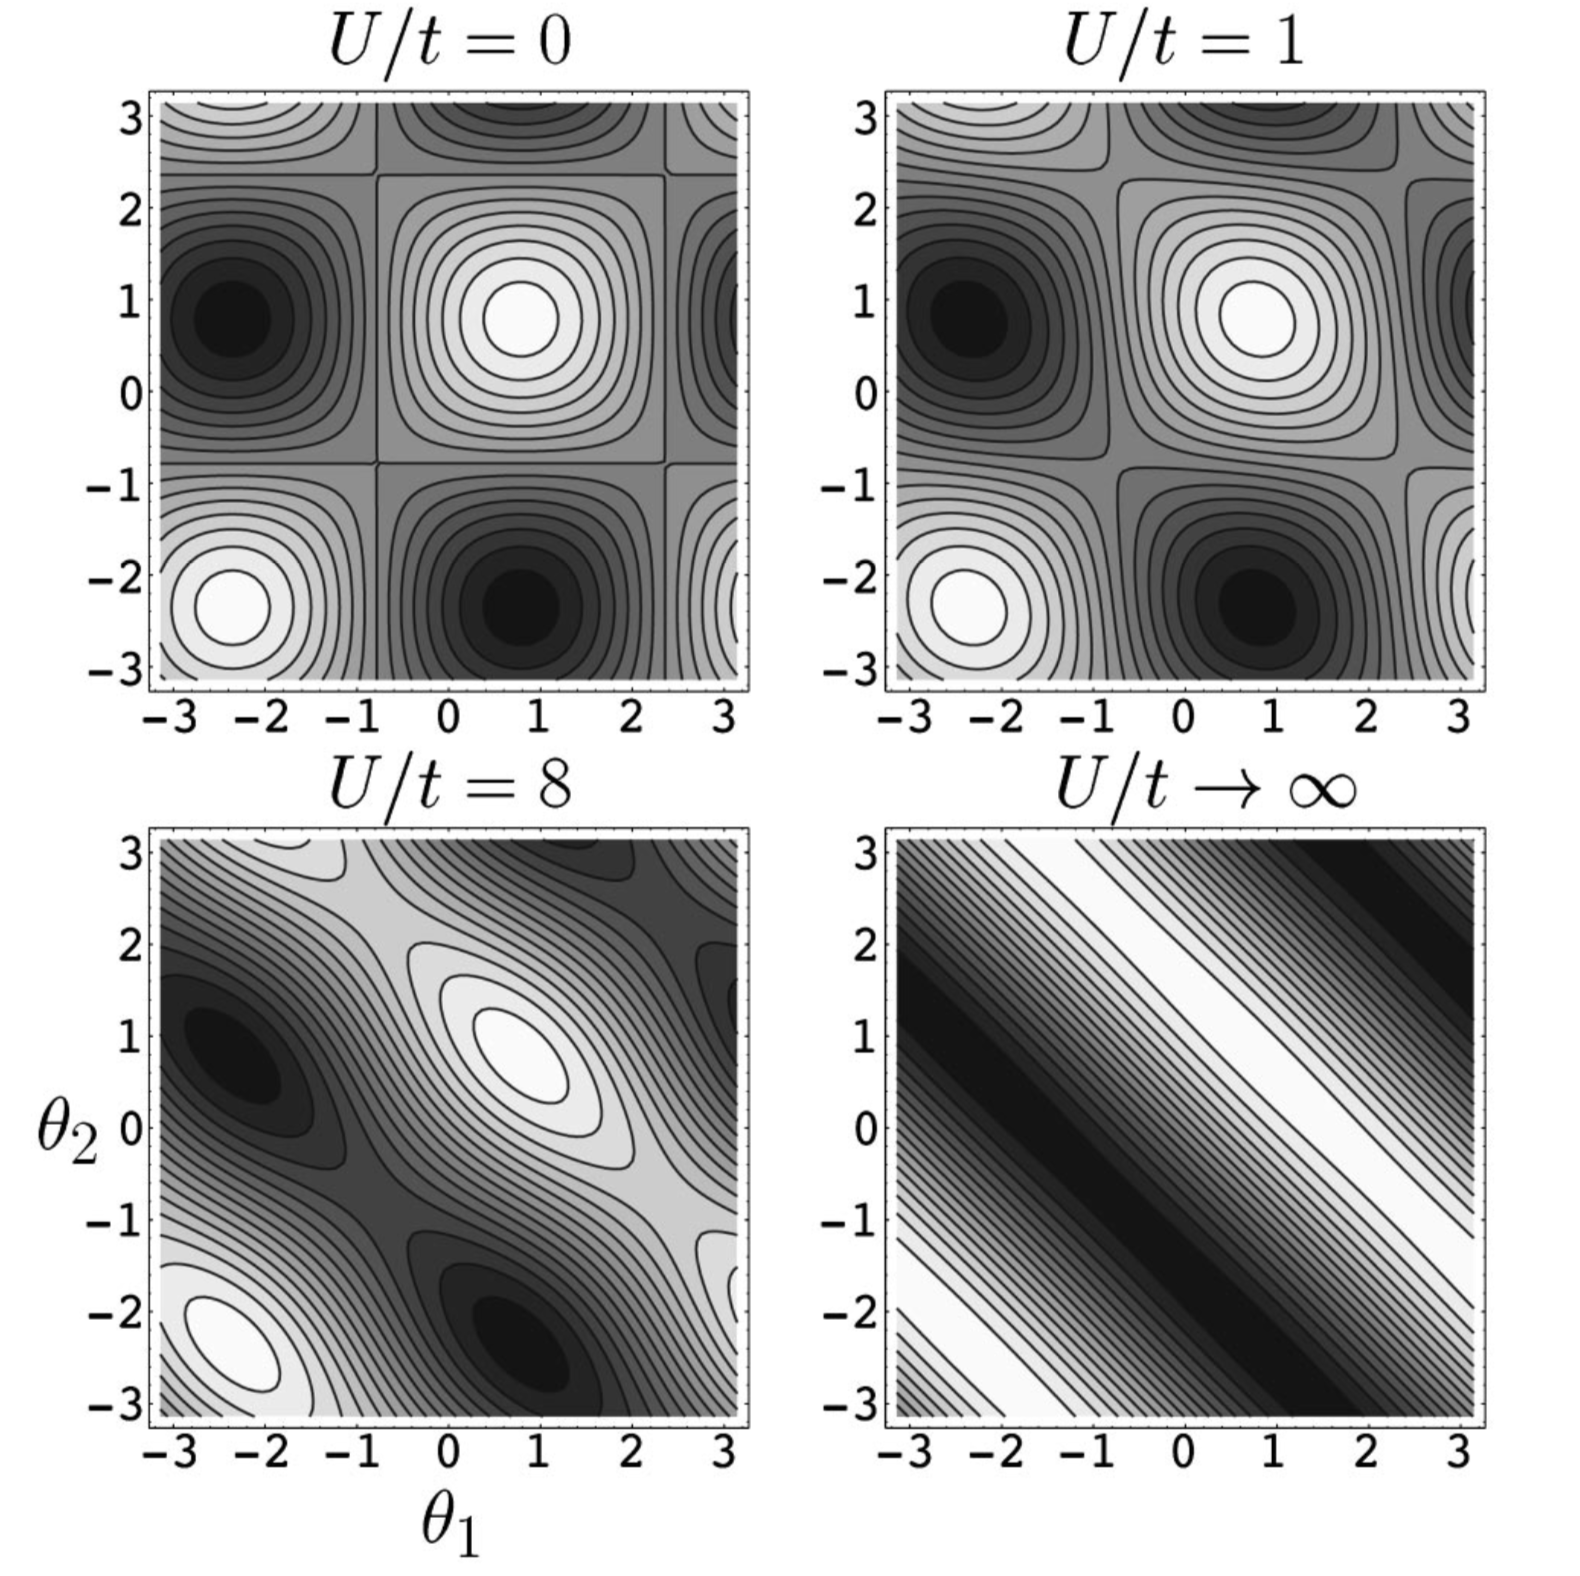
\includegraphics[width = 6cm]{constrained.png}
\caption{ Contour plots of the two-fermion ground state wave function overlap $<\chi | \phi_0 >$ for a Hubbard model as obtained in \cite{constrained2}. The parameters $\theta_{1,2}$ arise from the decomposition $|\chi > = (\cos\theta_1 c_{1\uparrow}^\dagger + \sin\theta_1 c_{2\uparrow}^\dagger) (\cos\theta_2 c_{1\downarrow}^\dagger + \sin\theta_2 c_{2\downarrow}^\dagger)$, where $c^{(\dagger)}$ are annihilation (creation) operators of two fermions with either spin up or down. Notice the varying nodal surfaces as the interaction energy-hopping parameter ratio varies. The accuracy of the constrained path QMC method depends on the shape of these surfaces (taken from \cite{constrained2}). }
\end{figure}

\subsection{Determinantal/Auxiliary Field QMC}\paragraph{}

The idea of this method is establish a mapping between quantum and classical Monte Carlo, using a suitable change of variables. The random variables are then sampled from the configuration space of the corresponding classical problem. The price to pay is that for a d-dimensional quantum problem, the corresponding classical problem is $(d+1)$-dimensional: an additional degree of freedom is added, and as we will show it corresponds to an imaginary time.

The expected value of a physical observable $\mathcal{O}$ may be written as $<\mathcal{O}> = Tr (\mathcal{O}\mathcal{P})$, where we have defined a projection operator

\begin{equation}
\mathcal{P} = \frac{1}{\mathcal{Z}}e^{-\beta\mathcal{H}} \, , \mathcal{Z} = Tr (e^{-\beta \mathcal{H}}) = \sum_i < \psi_i | e^{-\beta \mathcal{H}} | \psi_i > ,
\end{equation}
and the trace is taken over the Hilbert space describing all possible occupations in a lattice model.\par

Finding an approximation to the projection operator which is amenable to computation is done in terms of the Hubbard-Stratonovich transformation: the problem is  reformulated in terms of auxiliary variables $h_i$. The set $\{h_i\}$ is known as the Hubbard-Stratonovich field.\par

In the end, we sample configurations, that is, particular realizations of the HS field, with probability $P(h)$. It is the computation of this probability that requires determinant calculations giving the name to the method. For concreteness, we state without proof that for the example of the Hubbard model we have:

\begin{equation}
P(h) = \frac{\eta_d}{Z_h} \det [ M_{+}(h) ] \det [ M_{-}(h) ] ,
\end{equation}
where $M_\sigma (h)$ are fermion matrices depending on the imaginary time frame, spin, and the HS field; $\eta_d$ is simply a normalization constant depending on dimension, and $Z_h$ is the partition function expressed in terms of the HS field \cite{qmc}.

To move from a configuration $\{h\}$ to a new one $\{h'\}$, we vary, or flip, the value of only one variable $h_i$, leaving the rest unchanged. We use an acceptance-rejection scheme - the Metropolis-Hastings algorithm - that ensures that the accepted sample configuration follows the desired distribution. Once we reach equilibrium, i.e. the Markov Chain hits the stationary distribution, we have finished the so called warm up steps, and we may start measuring.\par

Recall the reasoning that was made in section \ref{subsec:dmc}. The solution of the Schr\"odinger equation may be expressed in terms of a linear combination of stationary states, which depend on time via a factor $e^{-iE_n t}$, where $n$ labels the energy level of the quantum system under study. We choose the energy scale so that all energies are positive and perform a change of variable to imaginary time $t= -i\tau$. The solution's time dependence is now described by a sum of transients $e^{-E_n \tau}, \, n \in \mathbb{N}$, and by following the (imaginary) time evolution of the wave function long enough, we will asymptotically reach the ground state energy $E_0$, and its corresponding wave function $\phi_0$. Note that this is independent of the initial condition in which we prepare the system. Convergence speed may eventually depend on this choice, but from a mathematical point of view if we wait long enough only the ground state will survive. The imaginary time many-body propagator $U(\tau) = e^{-H\tau}$ filters a trial wave function $\phi$ to the exact ground state $\phi_0$:

\begin{equation}
E_0 = \lim_{\tau \rightarrow \infty} \frac{<\phi | HU(\tau) | \phi >}{<\phi | U(\tau) | \phi >}
\end{equation}

We impose the condition that $\phi$ mustn't be orthogonal to $\phi_0$. Additionally, we require $\phi$ to be a symmetrized (antisymmetrized) product of single-particle orbitals for bosons (fermions).\par

The method can be used to treat systems with a variety of interactions. In general:

\begin{equation}\label{eq:general_h}
\mathcal{H} = \sum_{\alpha\beta} K_{\alpha\beta} \rho_{\beta\alpha} +\frac{1}{2} \sum_{\alpha\beta\gamma\delta} v_{\alpha\beta\gamma\delta} \rho_{\gamma\alpha} \rho_{\delta\beta} ,
\end{equation}
where $\rho_{\beta\alpha}\equiv a_\alpha^\dagger a_\beta$ and
$K_{\alpha\beta} = T_{\alpha\beta} \pm \frac{1}{2} \sum_{\gamma} v_{\alpha\gamma\gamma\beta}$
is the kinetic energy $T$ plus a self-interaction term for bosons or fermions, respectively. The subscripts ${\alpha, \beta, \gamma, \delta}$ represent eventually present degrees of freedom: spin, isospin, etc., as well as spatial coordinates \cite{sugiyama}.\par

We introduce an auxiliary field $h$ that reduces the exponential of the two-body operator in equation (\ref{eq:general_h}) to a functional integral over an infinite set of exponentials of one-body operators. We then run Monte Carlo to approximate these integrals. A valuable property of AFQMC is that it properly treats fermions: the HS representation of the propagator affords a description in terms of single-particle exactly antisymmetrized wave functions. GFQMC and DQMC do not share this property.\par

The long time behavior of a trial state: $\lim_{\tau \rightarrow \infty } e^{-\tau (\mathcal{H} - \varepsilon_0)} |\psi_T > = | \phi_0 > < \phi_0 | \psi_T >$ may be mapped onto a stochastic process in the manifold of N-particle Slater determinants $\mathcal{D}(N)$ \cite{zhang}. The mapping to a stochastic process is made possible by the discretization

\begin{equation}
e^{-\tau (\mathcal{H} - \varepsilon_0)} = (e^{-\delta \tau ( \mathcal{H} - \varepsilon_0 ) })^n \quad \text{with} \quad \delta \tau = \frac{\tau}{n}
\end{equation}

The HS transformation is in fact an operator identity that allows the establishment of a formal correspondence between a system of interacting fermions and an ensemble of non interacting fermion systems coupled to fluctuating external potentials. This leads to a random walk representation of the imaginary time evolution.\par

A limitation of the straightforward numerical implementation of AFQMC is that it leads to an exponential increase in statistical errors with imaginary time. This is due to the appearance of random complex phases during the evolution. To solve this problem, S. Zhang introduced an importance sampling transformation guiding the random walk \cite{zphase}  . This is done by introducing shift parameters in terms of which we rewrite $e^{-n\delta \tau (\mathcal{H} - \varepsilon_0)} |\psi_T >$. These parameters are chosen to minimize fluctuations in the importance function to first order in $\delta \tau$.\par

The aim is to solve the sign problem which arises when the overlap between one or more walkers and the trial state vanishes, yielding large fluctuations in the importance function, and generating statistical errors in AFQMC's estimates.

\subsection{Computational Complexity and the Sign Problem}

The sign problem afflicting many-fermion QMC causes an exponential increase of the computing time with the number of particles. A polynomially scaling algorithm would provide an unbiased and numerically exact solution (as in the case of bosons) for the problem of simulating a strongly correlated electron system. However, the problem was recently shown to be NP hard \cite{troyer}. Solving the sign problem would solve all NP problems in polynomial time (proving that $NP = P$) in what would be a major breakthrough in mathematics. This is widely believed to be unlikely, i.e. there is a conjecture that $NP \neq P$, although currently no mathematical proof exists of this impossibility.\par

Specific sign problems might be solvable. This indeed happens for a restricted subclass of quantum systems, for example see \cite{wiese, arnow,kalos}. An interesting open question is that of determining which models allow a partial solution of the sign problem due to their special properties. In particular, it is relevant for this field whether the 2D fermionic Hubbard model belongs to this class or not. A promising idea to circumvent NP hardness is to use ultracold atoms in optical lattices \cite{optical}, effectively using a quantum simulator to study the phase diagrams of correlated quantum systems. Although promising, even this method may not solve the problem in general: it is also still an open question whether a quantum computer could ever solve the NP complete problem (see \cite{troyer} and references therein).

\section{Comments on the references}
\begin{itemize}
\item \emph{Graphene and the rise of 2D materials} \cite{graphene, graphene_nobel} : review articles on the discovery of graphene and its properties. 
\item \emph{TMD nanoribbons - a new member of the 2D material family} \cite{tmd_family1, tmd_family2, tmd_family3} : reviews on the emergence of  TMD's, their electronic, magnetic, and structural properties, and prospects of future advances in nano and optoelectronics associated to the possible use of TMD's in applications.
\item \emph{Fabrication of TMD nanoribbons} \cite{chen} : discusses various experimental methods to fabricate $MoSe_2$ nanoribbons via an unusual morphological phase transition. The growth mechanism that is proposed could be applied to other TMD nanoribbons. It takes advantage of the temperature dependence of growth - the nanoribbons are obtained by increasing the temperature of a substrate - relying on shape transformations in nonequilibrium growth of surface-based nanostructures.
\item \emph{TMD nanoribbons and recent perspectives} \cite{nanoribbon,topological, tmd_magnetism} (and references therein) : recent studies in the stability of metallic edges in TMD nanoribbons, and the possibility of a superconducting phase arising in monolayer hole-doped TMD's, as well a computation of the valley/magnetic phase diagram of a monolayer hole-doped TMD, showing an instability towards an itinerant ferromagnetic phase. Valleys, i.e. degenerate valence band maxima, or conduction band minima, correspond to a degree of freedom that indicates the region of momentum space where charge carriers are confined. Carriers are then characterized not only by charge, and spin, but also by \emph{valley}, which can be used to control quantum states to generate novel devices in the framework of \emph{valleytronics}.
\item \emph{Emergence of magnetism in nanoribbons} \cite{yazyev} : this review covers the appearance of magnetic ordering in zigzag edges of graphene nanoribbons, and comments on possible applications. It also mentions some computational approaches, obtained results, and future prospects.
\item \emph{QMC results for graphene nanoribbons} \cite{qmc_results1, qmc_results2, qmc_results3, qmc_results4, qmc_results5} : Going beyond mean field, QMC has been used to investigate edge magnetism for a variety of situations in graphene, namely where strain is used to control the magnetic properties of zigzag edged nanoribbons.
\item \emph{Classical Monte Carlo} \cite{newman_barkema} : the  standard book widely used to learn the basics of classical Monte Carlo simulations in statistical physics, which are the same basic concepts used in QMC. The concepts of importance sampling, and detailed balance in the context of a Markov Chain MC are discussed.
\item \emph{Overview of aforementioned QMC methods} \cite{tao} : a recent book providing an overview of most QMC methods reviewed here. It was used throughout to learn the basic ideas of the various QMC methods.
\item \emph{A few existing QMC libraries} \cite{quest,montepython,alps,alf} : documentation of existing implementations of QMC in various programming languages.
\item \emph{Review of VQMC and DQMC} \cite{vmc_review,vmc,umrigar} : excellent review articles covering the basics of VQMC and DQMC, optimizing the trial wave functions used in VQMC. These include the concept of a variational state which is used as a starting point for QMC algorithms, and that of a diffusion Schr\"odinger equation in imaginary time. The latter is at the heart of DQMC, in the sense that all transient states, except the ground state vanish asymptotically as time goes by, which gives access to the ground state structure.
\item \emph{Path integral QMC and treating the sign problem} \cite{arnow,kosztin,constrained,constrained2, springer} : path integral formulation and improvements trying to circumvent the sign problem found in DMC. These shall be crucial in our project, once they give strategies to deal with the fermion sign problem which afflicts QMC methods applied to fermion interactions. A path integral formulation is not only of formal character. In fact, a very rich computational method arises out of it. Imposing certain conditions on the system's path in phase space allow us to control the sign problem.
\item \emph{Auxiliary Field and Phaseless Determinantal QMC} \cite{qmc,zhang,zphase} : main notes used for AFQMC and application to the Hubbard Model, phaseless AFQMC as an improved determinantal method. These articles contain the basics of determinantal QMC, and, once again, ways of combating certain numerical issues that arise in this context. 
\item \emph{The fermion sign problem is NP hard. An outlook} \cite{troyer, wiese,optical, arnow,kalos} : proof that the fermion sign problem is NP hard, models for which there is a solution to the sign problem, outlook on the future of QMC. Future perspectives on the method are presented, along with an estimate of its computational complexity. Interestingly enough, it is proved that finding a less complex QMC method for fermions would imply solving one of the most debated computer science problems we face nowadays.
\end{itemize}

\section{Work timeline}

This project will be carried out over a 20-week period. In this section we list tasks per week.
\vspace{10mm}
% #3 is yearcolumnwidth
% #4 is rulecolumnwidth
% #5 is entrycolumnwidth
% #6 is timelineheight
\begin{timeline}{1}{20}{0.5cm}{1cm}{6.5cm}{14cm}
\entry{1}{Review of Classical Monte Carlo}
\plainentry{2}{Build benchmarks for simple examples}
\entry{3}{Review of main 2D materials results and TMD's}
\entry{4}{Explore relevant QMC methods, start writing thesis}
\plainentry{5}{Review open source libraries, namely QUEST \cite{quest}, Alps \cite{alps}, Monte Python \cite{montepython}, ALF \cite{alf} }
\entry{8}{Implement QMC code, application to simple models}
\plainentry{10}{Determine which are the main quantities to measure for TMD nanoribbons}
\entry{12}{Implement measurements and test the code on more complex models}
\entry{16}{Start performing QMC measurements}
\entry{18}{Compile and interpret results}
\entry{20}{Finish writing thesis, review and editing}
\end{timeline}

\printbibliography

\end{document}
% %%%%%%%%%%%%%%%%%%%%%%%%%%%%%%%%%%%%%%%%%%%%%%%%%%%%%%%%%%%%%%%%%%%%%%
% The Introduction:
% %%%%%%%%%%%%%%%%%%%%%%%%%%%%%%%%%%%%%%%%%%%%%%%%%%%%%%%%%%%%%%%%%%%%%%
\fancychapter{Conclusions and Future Work}
\label{cap:conclusions}

Conclusions Chapter

\cleardoublepage
\cleardoublepage
\phantomsection
\addcontentsline{toc}{chapter}{Bibliography}
%% Use with Cite and Natbib
\bibliographystyle{IEEEtran}
\bibliography{02.biblio}
%% Use with Biblatex (.bib file is set in Packages) (Not working)
%\printbibliography

\cleardoublepage

\begin{appendices}
	\begin{appendix}
		\pagenumbering{bychapter}
		\fancychapter{Title of AppendixA}
\label{ap:a}

     
		\cleardoublepage
	\end{appendix}
\end{appendices}


\end{document}